% Consolidated project report. Build (from the folder report/):  pdflatex main.tex  (run twice for the table of contents and cross references)
\documentclass[11pt,a4paper]{article}
\usepackage[margin=2.3cm]{geometry}
\usepackage[T1]{fontenc}
\usepackage{lmodern}
\usepackage[utf8]{inputenc}
\usepackage{microtype}
\usepackage{amsmath,amssymb}
\usepackage{graphicx}
\usepackage{booktabs,longtable,array,tabularx,multirow}
\usepackage{xcolor}
\usepackage{float}
\usepackage[labelfont=bf,font=small]{caption}
\usepackage{enumitem}
\usepackage{url}
\usepackage{fancyhdr}
\usepackage{listings}
\usepackage{tikz}
\usetikzlibrary{positioning,arrows.meta,fit,shapes.geometric,calc,backgrounds}
\usepackage[colorlinks=true,linkcolor=blue!50!black,urlcolor=blue!50!black,citecolor=blue!50!black]{hyperref}

\definecolor{headlineblue}{HTML}{2A78D6}
\definecolor{baselineorange}{HTML}{EB6834}
\definecolor{ruleblack}{HTML}{8A8984}
\definecolor{softgreen}{HTML}{1BAF7A}
\definecolor{softred}{HTML}{E34948}

\DeclareRobustCommand{\code}[1]{\texttt{\detokenize{#1}}}   % code names (underscores allowed; robust so that it survives section titles and the table of contents)
\newcommand{\pth}[1]{\path{#1}}                   % file system paths (line-breakable)
\newcommand{\codename}[1]{(code name \code{#1})}
\newcommand{\todo}[1]{\textcolor{softred}{[#1]}}
\newcommand{\headline}{\emph{headline model}}

\lstset{basicstyle=\ttfamily\footnotesize,breaklines=true,frame=single,columns=fullflexible,keepspaces=true,
        showstringspaces=false,backgroundcolor=\color{black!3}}
\setlist{itemsep=2pt,topsep=3pt}
\setlength{\parindent}{0pt}
\setlength{\parskip}{5pt}
\sloppy
\emergencystretch=2em
\setcounter{tocdepth}{2}
\pagestyle{fancy}\fancyhf{}
\fancyhead[L]{\small Consolidated project report}
\fancyhead[R]{\small Camera-derived bird's-eye-view driving policies in MetaDrive}
\fancyfoot[C]{\thepage}
\renewcommand{\arraystretch}{1.12}

\title{\textbf{Camera-Derived Bird's-Eye-View Driving Policies in MetaDrive}\\[4pt]
\large Consolidated project report: where everything is, what every model is, how it was trained,\\
what worked, what did not, what failed and why, and which paper directions the evidence supports}
\author{Prepared for the project director\\ Written from the repository state of 11 November 2026}
\date{}

\begin{document}
\maketitle
\thispagestyle{empty}

\begin{abstract}
\noindent This document consolidates the whole project into one place. It explains the repository layout (including what is on the public
GitHub remote and what exists only on this machine), every trained model with its architecture, input, labels and training strategy,
the experimental protocol, all results that are supported by enough episodes to be reported, a dedicated account of every reinforcement-learning
attempt, a failure analysis, the front-camera videos recorded for one seed under several weather conditions, an assessment of which paper
directions are strongly supported by the evidence, and a verified list of related 2025--2026 papers on arXiv.

\medskip\noindent\textbf{Headline findings (all numbers are from 200 paired episodes unless stated otherwise).}
\begin{itemize}
\item The best learned model (the \emph{headline model}: dataset-aggregation student with a map-overlay bird's-eye view and three scalars) reaches
  \textbf{0.925} success in clear weather with sparse traffic, against \textbf{0.850} and \textbf{0.745} for the two behaviour-cloning baselines supplied in the
  repository (paired exact McNemar $p=0.0007$ and $p<0.0001$). It is statistically indistinguishable from the collision-aware rule-based teacher it imitates (0.950).
\item Under the weather perturbations that were measured and implemented, the headline model does \emph{not} get worse (0.89--0.91 in all four conditions), so
  \emph{no robustness or adaptation claim can be made}. The measured degradation of the detector and stereo depth is real (the detector finds 72\% of vehicles in clear weather and 1\% in heavy rain) but
  it hardly reaches the policy in sparse traffic.
\item Reinforcement learning did not improve on the imitation-trained policies in any of the four attempts documented here; one attempt made the policy significantly worse (0.815 versus 0.880 for its own starting point, $p=0.029$).
\item Failures of the headline model are concentrated in 15 of 200 episodes; in 14 of them the collision-aware teacher succeeds, so they are imitation failures, not intrinsically unsolvable scenes. Eight of the 15 end in the first 12 seconds.
\item A single seed (5169) was found on which both baselines crash in all four weather conditions while the headline model succeeds in all four; front-camera videos of it are described in Section~\ref{sec:videos}.
\end{itemize}
\end{abstract}

\newpage
\tableofcontents
\newpage

\section{Orientation: purpose, conventions and how to read this document}

\subsection{What this project is}
The project builds driving policies for the MetaDrive simulator that act from a \emph{bird's-eye view} (a top-down 64$\times$64 grid around the car, abbreviated BEV in the
code and in the teammates' documents, but written out here) plus a few scalar quantities, and asks how well such policies drive in traffic and when the
perception that feeds the grid is degraded by simulated fog and rain. The repository has three layers of work:
\begin{enumerate}
\item \textbf{Teammates' modules} (on the public GitHub repository): a vector-observation behaviour-cloning baseline, a five-camera rig with stereo depth, a YOLO object-detector with
  an image-space weather filter, the assembly of detections into the bird's-eye-view grid, and a behaviour-cloning policy on that grid.
\item \textbf{Policy-side work done in this project} (so far only on this machine, not on GitHub): fast camera-free environments, teacher policies, dataset-aggregation training,
  reinforcement-learning experiments, evaluation harnesses, perception measurements, diagnostics and recordings.
\item \textbf{This report} and the clean-up of the repository around it (Section~\ref{sec:cleanup}).
\end{enumerate}

\subsection{Naming conventions used in this document}
Names in the code were chosen quickly during experiments and are often abbreviations. In this document and in every figure and table, models and methods are
called by \emph{descriptive names}. Wherever a model also has a short code name (the name of its folder or of its result file), that code name is shown
once in typewriter font so that it can be found in the files. Table~\ref{tab:glossary} translates every abbreviation and code name that appears in the files.

\begin{table}[H]\centering\small
\caption{Glossary: abbreviations and code names used in file names, in the code and in earlier notes, with the full descriptive name used in this report.}
\label{tab:glossary}
\begin{tabularx}{\textwidth}{@{}>{\raggedright\arraybackslash}p{3.6cm}X@{}}\toprule
Code name or abbreviation & Meaning in this report\\\midrule
BEV & Bird's-eye view: a 64$\times$64 grid, 20\,m wide and 20\,m long (17.5\,m ahead of the car, 2.5\,m behind), cell size 0.3125\,m, centred on the ego car.\\
IDM / stock IDM & Intelligent driver model: MetaDrive's built-in rule-based car-following controller. Used as a teacher; it sees exact simulator positions of all vehicles.\\
SafeTeacher / \code{safe_teacher} & The collision-aware teacher: the intelligent driver model with lane changes switched off plus a predictive braking layer (Section~\ref{sec:teachers}).\\
BC / behaviour cloning & Supervised imitation of recorded expert actions (regression of steering and throttle).\\
DAgger / dataset aggregation & Iterative imitation: the learner drives, the teacher labels the states the learner visited, and the labelled states are added to the training set (Ross et al., 2011).\\
PPO / proximal policy optimisation & The reinforcement-learning algorithm used in every reinforcement-learning attempt.\\
HD map & High-definition map: here the lane centre line and the road boundaries read from the simulator's map; treated as a legitimate structured input.\\
\code{repo_bc_clear} & Baseline behaviour cloning, trained on five demonstrations \emph{without} traffic (\pth{bc_clear_5eps_without_traffic.pt}).\\
\code{repo_bc_sparse} & Baseline behaviour cloning, trained on five demonstrations \emph{with} sparse traffic (\pth{bc_sparse_traffic_5eps.pt}). The repository calls it the recommended starting checkpoint.\\
\code{base_a} & Dataset-aggregation student on the teammates' unmodified one-channel view and all six scalars (no map overlay).\\
\code{ov_both}, \code{ov_bev_only} & Map-overlay view with all six scalars / with no scalars. (\code{ov} = overlay.)\\
\code{ov_split} & \textbf{The headline model}: map-overlay view and three scalars (speed, route progress, distance to goal); the three lane-geometry quantities were moved from the scalars into the overlay.\\
\code{arch_bev_only}, \code{arch_scalar_only} & Input-ablation models: view only / scalars only (\code{arch} = architecture ablation).\\
\code{caut_a}, \code{ctrl_nocaut}, \code{caut_c0}, \code{caut_auto} & Caution study: caution-conditioned network; its control with the caution input always zero; the same conditioned network evaluated with caution 0 and with caution derived from weather.\\
\code{deg_base} & Dataset-aggregation student trained under the calibrated degraded perception.\\
\code{ppo_plain}, \code{ppo_ada} & Reinforcement learning from \code{deg_base} without / with a weather input (\code{ada} = adaptive; this run did not finish).\\
\code{rl_plain}, \code{rl_energy}, \code{rl_safe}, \code{rl_head}, \code{rl_full} & Reward-combination sweep, reinforcement learning from the headline model (base reward; plus energy; plus safe-speed and scaled crash penalty; plus headway; all terms).\\
\code{C2}, \code{C3}, \code{probe_C}, \code{pilot_cond} & Early reinforcement-learning attempts (privileged teacher trained with PPO).\\
\code{pose_aug_*}, \code{pose_cam_*} & Pose-error study: map-pose-error augmentation (and two-cue variant with a noisy lane detector), conditioned or not on the error level.\\
\code{vcam} & Pixel policy: a small convolutional network that sees only a front-camera image.\\
Seed / seed block & Integer that selects the MetaDrive map, route and initial traffic. Disjoint blocks are used for training, validation and testing (Table~\ref{tab:seeds}).\\
Density & MetaDrive \code{traffic_density}: probability-like parameter controlling the amount of traffic. 0.05 = sparse, 0.2 = dense.\\
Wh/km & Estimated traction energy per kilometre from the declared virtual-vehicle model in \pth{bev_rl/energy.py}; not battery electricity.\\\bottomrule
\end{tabularx}
\end{table}

\subsection{Evidence levels}
Every quantitative statement in the document carries its sample size. Three levels are used:
\textbf{reported} ($n\ge 200$ paired episodes, confidence intervals and paired tests given),
\textbf{pilot} ($n=10$ to $40$ episodes; wide intervals; used to choose what to run next, not to claim),
\textbf{diagnostic} (one or two replayed episodes that explain a mechanism but do not measure a rate).

\subsection{How to read the document}
Sections~\ref{sec:repomap}--\ref{sec:perception} explain the setting; Sections~\ref{sec:arch}--\ref{sec:catalogue} describe the models; Sections~\ref{sec:headline}--\ref{sec:failure}
give the results and failures; Section~\ref{sec:videos} describes the videos; Section~\ref{sec:lessons} summarises what worked and what did not; Section~\ref{sec:directions} lists
paper directions and the evidence behind each; Section~\ref{sec:related} lists related 2025--2026 papers. Appendix~\ref{app:inventory} lists every file created or changed, and
Appendix~\ref{app:honesty} lists known defects and invalid runs.

\section{Repository map: where everything is}\label{sec:repomap}

\subsection{The GitHub remote}
The folder \pth{D:/bev_Fresh/bevcapstone} is a git repository with one remote, \code{origin} $=$ \url{https://github.com/Swathi-Srini/bevcapstone}. Checked on 11 November 2026:
\begin{itemize}
\item The local branch \code{main} is up to date with \code{origin/main} (after a fetch). The last commit on the remote is dated 8 September 2026 (``Merge pull request \#11: Add sparse traffic BC handoff baseline'').
\item The remote has eleven branches (\code{main}, \code{bev-bc-nominal-baseline}, \code{camera}, \code{docs/consolidate-readmes}, and six \code{rachana/*} branches for camera-stereo fixes, ground-truth validation of the stereo depth, and the YOLO-weather audit, hand-off and test suite).
  All of them are already merged into \code{main} except for one commit on \code{rachana/stereo-ground-truth-validation} that only removes generated camera captures; \emph{nothing of substance on the other branches is missing locally}.
\item The repository history has 40 commits. The tracked content is 120 files, 56 of which are saved camera frames; the rest is the teammates' code and documentation listed in Table~\ref{tab:teammates}.
\item \textbf{Nothing produced in this project's policy-side work has been committed or pushed.} All of \pth{bev_rl/}, the tests \pth{tests/test_bev_rl_*.py}, the three trained models of the earlier camera-view-version-2 experiment, this report and the trained-model folder are untracked. Three tracked teammate files are modified locally (next subsection).
\item \code{.gitignore} excludes \code{*.npz} demonstrations, all video files, every \code{runs/} folder and \code{logs/}. The new folder \pth{trained_models/} is \emph{not} ignored (model files are small: 35\,MB in total), but \pth{report/videos/} is ignored because of the \code{*.mp4} rule.
\end{itemize}

\begin{table}[H]\centering\small
\caption{What the teammates' modules on the GitHub repository contain (read from the repository files and their README files).}
\label{tab:teammates}
\begin{tabularx}{\textwidth}{@{}>{\raggedright\arraybackslash}p{3.6cm}X@{}}\toprule
Folder & Content\\\midrule
\pth{baseline/bc_metadrive/} & Preserved comparison experiment: 259-dimensional MetaDrive vector observation, multilayer-perceptron behaviour cloning. Not used by this project's results; kept untouched.\\
\pth{camera/} & Five-camera MetaDrive rig (front-left and front-right stereo pair, left, right, rear) with capture script and a front depth map from semi-global block matching; 80 example frames are tracked.\\
\pth{YOLO+weather module/} & Live YOLO version 8 object detection on the camera views, \emph{image-space} synthetic fog and rain (\pth{weather/weather_utils.py}), reusable stereo depth (\pth{stereo_depth/}), a ground-truth stereo benchmark and a unit-test suite.\\
\pth{bev_state/} & Assembles detections and depth into the 64$\times$64 grid and the six-dimensional scalar state (class \code{BEVStateAssembler}; grid encoding: $-1$ unknown, 0 free, 0.5 route, 0.8 road boundary, 0.9 ego, 1.0 detected vehicle).\\
\pth{bev_policy/} & Behaviour-cloning policy (CNN on the grid + multilayer perceptron on the scalars), demonstration collector, evaluator, metrics, plotting and the two baseline checkpoints.\\
\pth{tests/} and \pth{.github/workflows/} & Unit tests for the grid assembly and metrics; a GitHub Actions workflow that verifies the repository on Windows with Python 3.11.\\
\pth{docs/} & The architecture specification (\pth{AV_Carla_BEV (1).pdf}) that fixes the grid layout, values and reward structure.\\\bottomrule
\end{tabularx}
\end{table}

\subsection{Teammates' files that were modified locally}
The root \pth{README.md} was edited on 11 November 2026 (a ``Start here'' pointer to this report and the new folder layout; all of the teammates' text is kept). In addition, three tracked files in \pth{bev_policy/} carry uncommitted changes (\texttt{git diff} shows +56 / $-$17 lines). All three add an \emph{optional} weather-input branch and are backwards compatible
(the defaults reproduce the original behaviour, and the two baseline checkpoints load unchanged):
\begin{itemize}
\item \pth{bev_policy/model.py}: class \code{BEVScalarPolicy} gained the argument \code{weather_dim} (default 0). When positive, a one-layer encoder maps a weather vector to 16 features that are concatenated before the action head. Without it, the network is exactly the original.
  This branch is later reused as a generic ``extra input'' for the caution, pose-error and weather-aware models.
\item \pth{bev_policy/dataset.py}: loading of a stored weather array and of unsigned 8-bit grids; optional return of the weather vector.
\item \pth{bev_policy/train_bc.py}: options \code{--weather-input}, \code{--only-clear} and \code{--val-count} for the early camera-view-version-2 experiments.
\end{itemize}

\subsection{Layout after the clean-up}\label{sec:cleanup}
The repository was reorganised on 11 November 2026 at the project director's request. No code module was renamed (the evaluation scripts import each other by module name and the names are
recorded in this report instead), no teammate file was moved, and nothing was deleted except the superseded videos (see below).
Figure~\ref{fig:tree} shows the result; the following rules explain it.

\begin{figure}[H]
\small
\begin{lstlisting}[frame=single,basicstyle=\ttfamily\scriptsize]
bevcapstone/
|-- README.md                      project overview (teammates' text + pointer to this report)
|-- report/                        THIS REPORT: main.tex, sections/, figures/, tables/, data/, videos/, make_*.py
|-- trained_models/                ALL final trained models in one folder (copies) + MODEL_MANIFEST.json
|   |-- 01_baseline_behaviour_cloning/       the teammates' two baselines
|   |-- 02_superseded_early_experiments/     early camera-view-version-2 models (not used for results)
|   |-- 03_dataset_aggregation_students/     headline model, ablations, caution, pose-error, degraded-perception students
|   |-- 04_reinforcement_learning/           every reinforcement-learning checkpoint that was kept
|   |-- 05_camera_pixel_policy/              the image-only control policy
|   |-- 06_third_party_perception/           YOLO version 8 nano weights (not trained here)
|   `-- training_records/                    log.json / best.json / config.json of every run
|-- bev_policy/  bev_state/  camera/  baseline/  YOLO+weather module/   teammates' modules (see Table 2)
|-- bev_rl/                        policy-side code of this project (environments, teachers, training, evaluation, diagnostics)
|   `-- adaptive/                  all experiments of the dataset-aggregation / caution / degraded-perception phase
|       |-- runs/                  training workspace: every iteration of every run (kept: scripts read best.pt here)
|       |-- results/               evaluation result files (json/csv), per-episode outcomes
|       `-- logs/                  text logs of training and evaluation runs
|-- repository_tools/              scripts that organise the repository (copy models, ...)
|-- tests/                         teammates' tests + tests/test_bev_rl_*.py (policy-side tests)
|-- docs/                          specification pdf; project_history/ = earlier notes (dated names)
|-- archive/                       material kept for the record but not needed: earlier paper drafts, removed scripts, early runs
|-- logs/                          queue and recording logs
|-- weights/                       third-party YOLO weights used by the perception code
`-- requirements.txt, requirements-lock.txt, venv/
\end{lstlisting}
\caption{Repository layout after the clean-up of 11 November 2026.}\label{fig:tree}
\end{figure}

\paragraph{Rules applied.}
\begin{enumerate}
\item \textbf{All models in one folder.} \pth{trained_models/} holds a copy of the \emph{selected} checkpoint of each of the 33 models, named by what the model is (not by the folder it was trained in), together with
  the training records and a manifest (\pth{MODEL_MANIFEST.json}) that gives, for each file, the original path, the SHA-256 hash, the size and a plain-language description. The originals stay in \pth{bev_rl/adaptive/runs/} because the evaluation scripts load
  \pth{runs/<run>/best.pt}; those folders also contain every intermediate iteration and are treated as the training workspace, not as a place to look for models.
\item \textbf{Figures.} The report's figures are regenerated from the saved result files by \pth{report/make_report_figures.py}; the 42 figures of the earlier drafts were archived, not edited (Section~\ref{sec:figclean}).
\item \textbf{Videos.} The 146 earlier videos (about 1.2\,GB: top-down and bird's-eye-view panels, laggy camera panels, and a front-camera set at a different seed) were deleted and replaced by the front-camera recordings of Section~\ref{sec:videos}.
\item \textbf{Old notes.} The six notes in the repository root (architecture, decisions, experiment log, known limitations, preliminary literature review, research plan, all written in the first week of November) moved to \pth{docs/project_history/}
  with dated names; the folder \pth{research_log/} moved there as well.
\item \textbf{Superseded material.} The earlier paper folder (\pth{paper/}, including the draft in IEEE format and the hand-off documents) and the folder \pth{_to_delete_review_2026-11-05/} are in \pth{archive/}. Nothing in \pth{archive/} is imported by any code.
\end{enumerate}

\subsection{Figures: which are needed and which are not}\label{sec:figclean}
The earlier drafts accumulated 42 figure files in seven folders with duplication (the same headline chart existed twice) and with colour schemes that changed from figure to figure.
All of them are now in \pth{archive/paper_earlier_drafts/}. The report uses fifteen figures, listed in Table~\ref{tab:figures}, each generated from the saved result files (and not drawn by hand) with one colour per role:
\textcolor{headlineblue}{\textbf{blue}} = the headline model and its variants, \textcolor{baselineorange}{\textbf{orange}} = the two baseline behaviour-cloning models, \textcolor{ruleblack}{\textbf{grey}} = rule-based teachers that see simulator truth,
violet and pink = other learned models; green, red, yellow and grey in the outcome charts always mean success, collision, left the road and timeout.

\begin{table}[H]\centering\small
\caption{The figures of this report and what each one is for.}\label{tab:figures}
\begin{tabularx}{\textwidth}{@{}>{\raggedright\arraybackslash}p{6.6cm}X@{}}\toprule
File in \pth{report/figures/} & Purpose\\\midrule
\pth{fig_headline_success_clear_weather_200_episodes} & The main result: success with confidence intervals for six models.\\
\pth{fig_outcome_breakdown_200_episodes} & How each model fails (collision, left the road, timeout).\\
\pth{fig_per_episode_outcome_strips} & Which episodes each model fails; shows that failures overlap.\\
\pth{fig_paired_difference_headline_versus_others} & Paired differences with intervals (the statistical comparison).\\
\pth{fig_speed_versus_energy_200_episodes} & Speed and estimated energy of each model.\\
\pth{fig_measured_perception_degradation} & Measured detector and stereo-depth degradation under fog and rain.\\
\pth{fig_success_by_weather_calibrated_perception_200_episodes} & Success per weather condition for four models.\\
\pth{fig_success_versus_localisation_error} & Sensitivity to an error in the car's pose against the map.\\
\pth{fig_dataset_aggregation_validation_curves} & Validation success per training round for five input designs.\\
\pth{fig_reinforcement_learning_validation_curves} & Validation success during the reinforcement-learning runs.\\
\pth{fig_teacher_ceiling_dense_traffic} & Success of the rule-based teachers in dense traffic.\\
\pth{fig_birds_eye_view_fidelity_before_collision} & True gap versus the gap drawn in the grid before two collisions.\\
\pth{fig_success_versus_localisation_error_pose_trained_models} & Effect of training with pose error and of a second lane cue.\\
\pth{fig_birds_eye_view_input_examples} & The two grid encodings drawn from a real scenario.\\
\pth{fig_seed5169_front_camera_frames} & Frames of the recorded videos (Section~\ref{sec:videos}).\\\bottomrule
\end{tabularx}
\end{table}

\section{Experimental setup}\label{sec:setup}

\subsection{Simulator, scenarios and outcomes}
All experiments use MetaDrive version 0.4.3 (pinned in \pth{requirements.txt}) on a CPU laptop. A scenario is determined by an integer \emph{seed} that selects a procedurally generated road network (random number of lanes and
lane width, intersections and roundabouts occur), the route to the destination, the initial position of the ego car and the initial positions of the traffic vehicles. The decision frequency is 10\,Hz. An episode ends with exactly one outcome:
\begin{description}[leftmargin=3.2cm,style=nextline]
\item[success] the ego car arrives at the destination (MetaDrive flag \code{arrive_dest});
\item[collision] any of the flags \code{crash_vehicle}, \code{crash_object}, \code{crash_building}, \code{crash_human};
\item[left the road] the flag \code{out_of_road} (also triggered by leaving the planned route);
\item[timeout] the horizon (800 steps $=$ 80\,s in all evaluations, 600 steps during dataset-aggregation training) is reached without one of the above.
\end{description}
Traffic is controlled by the density parameter: \textbf{0.05 (sparse)} for all reported results, \textbf{0.2 (dense)} for diagnostics. The action contract is MetaDrive's two-dimensional action
\code{[steering, throttle/brake]} in $[-1,1]^2$. The rule-based driver (stock intelligent driver model) cruises at about 8.3\,m/s (30\,km/h), so the mean speeds in this report are 7--9\,m/s.

\subsection{Why the policies do not run on live camera pixels}\label{sec:surrogate}
The teammates' full perception chain renders five cameras at 1200$\times$900, runs YOLO on the views, estimates depth with stereo block matching and assembles the grid. Measured on this laptop it costs 1.7--2.5\,s per step
(about 4\,GB of memory; Section~\ref{sec:perception}), which makes training and 200-episode evaluations infeasible. The policy-side work therefore uses a \textbf{camera-free surrogate environment} (\pth{bev_rl/adaptive/env.py}, class \code{AdaptiveEnv} and its subclasses):
\begin{itemize}
\item The grid is built by the teammates' \emph{unmodified} function \code{build_bev_grid} from the list of vehicles that MetaDrive reports inside the grid window (an ideal detector), with the ego footprint and unknown/free cells as in the teammates' encoding.
\item The scalar state is the same six-dimensional vector \code{[speed, route progress, lateral offset, heading error, curvature ahead, distance to goal]}.
\item \textbf{Weather} acts only through perception. It never changes the vehicle dynamics or tyre friction in any reported result. Two stand-ins for the perception loss are used: (i) \emph{detector dropout}, where each vehicle is removed from the grid with probability one minus the measured detector retention
  for that weather; (ii) \emph{calibrated degradation}, built from the measurement of Section~\ref{sec:perception}, where a vehicle can additionally be displaced because of a wrong stereo range.
\item The equivalence of the optimised perception path with the original path was tested (\pth{bev_rl/validate_lazy_perception.py}; notes in \pth{docs/project_history/research_log_2026-11-01_environment_and_audit/04_LAZY_PERCEPTION_EQUIVALENCE.md}): 70 of 70 frames were bit-identical, \emph{but only one of those frames contained an occupied grid cell}, so the stereo branch was exercised rarely; the evidence is weak and is listed as a limitation (Appendix~\ref{app:honesty}).
  A cached free-space mask used for speed was found identical to \code{build_bev_grid} over 400 grids.
\end{itemize}
\textbf{Consequence for claims:} what is reported here is the quality of the \emph{policies given a perception model}, not of the end-to-end camera system. The front-camera videos (Section~\ref{sec:videos}) therefore show the camera frames next to the policy's behaviour but the policies do not read those pixels.
One exception: the pixel policy \code{vcam} (Section~\ref{sec:catalogue}) does read camera frames.

\subsection{Seed blocks}
Disjoint blocks of seeds are used so that no evaluation scenario was used for training, validation or model selection (Table~\ref{tab:seeds}).
\begin{table}[H]\centering\small
\caption{Seed blocks and their use. Seeds 5000--5003 were additionally used once for a superseded early pilot of the camera-view-version-2 models (a development run, never used to select any reported model).}\label{tab:seeds}
\begin{tabularx}{\textwidth}{@{}l>{\raggedright\arraybackslash}X@{}}\toprule
Seeds & Use\\\midrule
2000--2999 & Training scenarios for dataset aggregation and reinforcement learning.\\
3000--3003 & Calibration of the earlier surface classifier (camera-view-version-2 experiment, superseded).\\
3100--3139 & Validation: choice of the best training round (3100--3109 for dataset aggregation; 3100--3139 for reinforcement learning with reward version 3).\\
1000--1009 & First reserved test block ($n=10$): input-ablation pilot.\\
1010--1049 & Second test block ($n=40$): caution, localisation-error and detector-dropout pilots.\\
\textbf{5000--5199} & \textbf{Final test block ($n=200$)}: every reported number in Sections~\ref{sec:headline}--\ref{sec:weather} unless stated.\\
7000--7039 & Measurement of the detector and stereo degradation (Section~\ref{sec:perception}).\\
4000--4039 & Early demonstrations of the superseded camera-view-version-2 experiment.\\\bottomrule
\end{tabularx}
\end{table}

\subsection{Metrics}
\begin{itemize}
\item \textbf{Success rate} with the 95\% Wilson score interval, and the shares of collision, left-the-road and timeout.
\item \textbf{Mean speed} (m/s) and \textbf{route completion} (fraction of the route driven; 1.0 at the destination).
\item \textbf{Estimated traction energy} in watt-hours per kilometre (\pth{bev_rl/energy.py}). It is the mechanical work at the wheels for a declared virtual vehicle (drag coefficient 0.23, frontal area 2.22\,m$^2$, rolling resistance 0.01, mass from the simulator vehicle), integrated exactly
  for linear speed change within each 0.1\,s step, with no regenerative braking and no gradient. It is \emph{not} battery electricity and not a MetaDrive quantity; only differences between models are meaningful.
\item \textbf{Paired comparison.} Because every model is evaluated on the same 200 seeds, two models are compared with the exact McNemar test on the discordant episodes and a 5000-sample paired bootstrap interval of the difference in success rates. This is much more powerful than comparing two overlapping Wilson intervals.
\end{itemize}

\subsection{Reproducibility caveat}\label{sec:repro}
A replay of the same model on the same seed in different process histories can give different episodes: the map, route, ego pose and initial traffic positions are identical, but the traffic random-number generator is not reseeded at reset, so traffic behaviour can diverge
(base model, seed 1012: 638 steps alone, 510 steps after seed 1040, 509 after seed 1039, a crash at 374 steps in a video run). Repeating the \emph{same evaluation order in a fresh process} is reproducible; comparing across different run orders is not exact.
This matters for the videos (Section~\ref{sec:videos}), where outcomes were re-checked rather than assumed.

\section{What fog and rain do to the perception: the measurement}\label{sec:perception}

\subsection{Why it was measured}
The teammates' weather module corrupts the camera images (Koschmieder-style fog with per-pixel depth, alpha-composited rain streaks), and the stereo depth that places a detected vehicle in the grid is computed from the corrupted image pair.
An earlier policy-side proxy removed vehicles from the grid at random with a probability taken from an older measurement of the detector (``detector dropout''). Every policy was completely flat under that proxy, so no claim about adaptation could be tested.
The project director's position was that weather also degrades the \emph{depth}; this had to be measured before anything was trained on it. The measurement (\pth{bev_rl/adaptive/measure_depth_error.py}) only \emph{calls} the teammates' functions
(\code{apply_synchronized_stereo_weather}, \code{front_stereo_depth}, \code{object_stereo_depth}, \code{run_yolo}, \code{project_world_point}) and compares with the MetaDrive ground truth; it modifies nothing in the teammates' modules.
Hypotheses and decision rules were written down \emph{before} the measurement (\pth{report/data/preregistration_depth_degradation.md}).

\subsection{Protocol}
Seeds 7000--7039 (40 scenes, traffic density 0.3), stationary ego car, traffic vehicles placed 5--19\,m ahead, each scene perceived clean and with two random weather draws per condition. Conditions: clear, fog 0.6, 0.8, 1.0 and rain 0.3, 0.6, 1.0
(the number is the intensity parameter of the teammates' augmentation). For every vehicle in view the following were recorded: whether YOLO detected it, whether the stereo depth at the vehicle's pixel was valid, and the range error of the box depth.

\subsection{Result}
\begin{figure}[H]\centering
\includegraphics[width=\textwidth]{figures/fig_measured_perception_degradation.pdf}
\caption{Measured perception degradation (40 scenes, 72 vehicle-frames in clear weather and 144 in each weather condition). Left: share of vehicles the YOLO detector finds, with 95\% Wilson interval. Right: share of vehicle pixels at which the stereo block matching returns a valid depth.}
\label{fig:perception}
\end{figure}

\begin{itemize}
\item \textbf{Detection collapses with weather} (hypothesis H0 in the pre-registration is confirmed): 0.72 in clear weather, 0.72 in fog 0.6, 0.59 in fog 0.8, 0.31 in fog 1.0, 0.57 in rain 0.3, 0.15 in rain 0.6 and 0.014 in rain 1.0.
\item \textbf{Stereo depth validity drops in fog} (0.88 clear, 0.63 in fog 0.8, 0.49 in fog 1.0) but much less in rain (0.81 at rain 0.6, 0.67 at rain 1.0).
\item \textbf{For vehicles that are detected, the range estimate does not get worse}: the box depth was valid for 100\% of detections in every condition and the median absolute depth error is \emph{lower} in fog and rain (0.98\,m clear, 0.36\,m fog 1.0, 0.67\,m rain 1.0). The share of detections with a relative error above 20\% does not rise (0.096 clear; 0.091 at fog 1.0; 0 in rain).
  The likely explanation is a selection effect (hypothesis, not tested): only close, large vehicles survive detection in heavy weather.
\item Consequently the degradation that reaches a policy is almost entirely \emph{missed detections}, and the ``wrong range'' branch of the calibrated environment is rarely triggered. This is the reason why even the calibrated degradation does not hurt the policy in sparse traffic (Section~\ref{sec:weather}).
\end{itemize}

\subsection{Consistency with the earlier retention table}
The detector-dropout proxy used a retention table measured earlier (\pth{bev_rl/adaptive/results/retention_table.json}): fog 1.0, rain 0.6 and rain 1.0 keep 0.27, 0.16 and 0.04 of the vehicles. The corrected measurement above gives 0.31, 0.15 and 0.014, i.e.\ the same order of magnitude;
the table's bias suspected after the stale-camera error (below) therefore seems small for these three conditions, but it has not been re-fitted.

\subsection{An invalid first measurement (kept for the record)}
The first run of the measurement (20:31--20:52 on 10 November) was \textbf{invalid}. It called a helper that mounts the camera rig \emph{once per environment object} after every reset, so scenes 2--40 had stale cameras: stereo depth was valid for only 2 of 73 clean vehicle-frames and was identical in all weather conditions.
The teammates' own benchmark script remounts the rig after every reset; the corrected run does the same. The invalid outputs were renamed \code{*.SUSPECT_*} and are kept; the pipeline stage (\code{hurt}) that had already used the invalid model was discarded and rerun. The same helper had been used by the earlier measurement that produced the retention table, which is why that table carries a caveat.
\emph{Lesson:} a perception measurement must be validated by an ``is the effect identical across conditions'' check before use.

\subsection{Cost of the full perception chain}
Benchmark of the teammates' chain (30 steps, seed 1000, no traffic): full resolution 1200$\times$900 with YOLO costs 1.7\,s (clear), 2.1\,s (fog 0.6), 2.5\,s (rain 0.6) per step; rendering the cameras at 600$\times$450 with a cached fog transmission, a cropped morphology region and YOLO disabled when there is no traffic
brings this to 0.20, 0.39 and 0.52\,s. Road-surface accuracy of the half-resolution variant was comparable (0.946 versus 0.945). Even so, a 100\,000-step reinforcement-learning run through this chain would take 50 hours or more, which is why the camera-free surrogate is used (Section~\ref{sec:surrogate}).

\section{Model architecture}\label{sec:arch}

All learned driving policies in this project share \emph{one} network family, the teammates' \code{BEVScalarPolicy} (\pth{bev_policy/model.py}). The models differ in \emph{what they are given as input}, \emph{who labels their training data} and \emph{how they are trained},
not in the network. This is deliberate: it makes the comparison between models a comparison between input designs and training strategies. The one different network is the image-only pixel policy (Section~\ref{sec:catalogue}).

\subsection{The shared network}
\begin{figure}[H]\centering
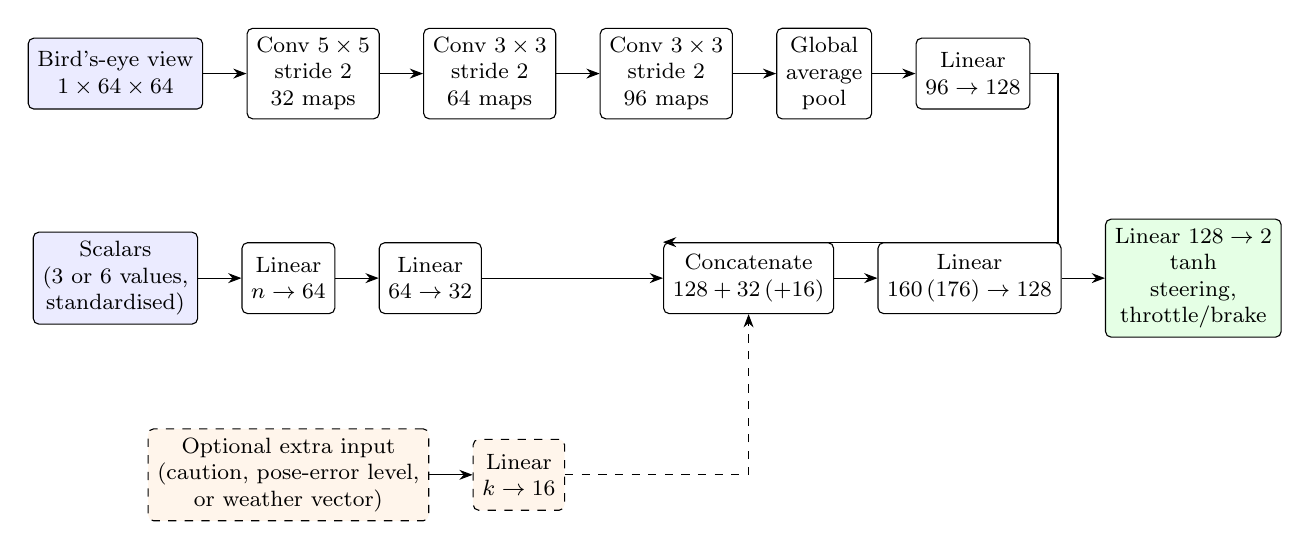
\begin{tikzpicture}[font=\footnotesize,>=Stealth,
  box/.style={draw,rounded corners=2pt,minimum height=0.9cm,align=center,fill=white},
  inbox/.style={box,fill=blue!8},
  optbox/.style={box,dashed,fill=orange!8},
  outbox/.style={box,fill=green!10},
  node distance=0.45cm and 0.55cm]
\node[inbox] (bev) {Bird's-eye view\\ $1\times64\times64$};
\node[box,right=of bev] (c1) {Conv $5\times5$\\ stride 2\\ 32 maps};
\node[box,right=of c1] (c2) {Conv $3\times3$\\ stride 2\\ 64 maps};
\node[box,right=of c2] (c3) {Conv $3\times3$\\ stride 2\\ 96 maps};
\node[box,right=of c3] (gp) {Global\\ average\\ pool};
\node[box,right=of gp] (l1) {Linear\\ $96\to128$};
\node[inbox,below=1.55cm of bev] (sc) {Scalars\\ (3 or 6 values,\\ standardised)};
\node[box,right=of sc] (s1) {Linear\\ $n\to64$};
\node[box,right=of s1] (s2) {Linear\\ $64\to32$};
\node[optbox,below=1.45cm of s1] (ex) {Optional extra input\\ (caution, pose-error level,\\ or weather vector)};
\node[optbox,right=of ex] (e1) {Linear\\ $k\to16$};
\node[box,right=2.3cm of s2] (cat) {Concatenate\\ $128+32\,(+16)$};
\node[box,right=of cat] (h1) {Linear\\ $160\,(176)\to128$};
\node[outbox,right=of h1] (o) {Linear $128\to2$\\ tanh\\ steering,\\ throttle/brake};
\foreach \a/\b in {bev/c1,c1/c2,c2/c3,c3/gp,gp/l1,sc/s1,s1/s2,ex/e1,cat/h1,h1/o} \draw[->] (\a) -- (\b);
\draw[->] (l1.east) -- ++(0.35,0) |- (cat.north west);
\draw[->] (s2) -- (cat);
\draw[->,dashed] (e1.east) -| (cat.south);
\end{tikzpicture}
\caption{The shared policy network. Each box is one layer; every layer except the last is followed by a rectifier. The dashed boxes exist only in the models with an extra input.
Parameter count: 110\,530 without the extra input and 112\,610 with a one-dimensional extra input.}
\label{fig:network}
\end{figure}

\paragraph{Inputs.}
\begin{description}[leftmargin=3.4cm,style=nextline]
\item[Bird's-eye view] A $64\times64$ grid covering 10\,m to each side, 17.5\,m ahead and 2.5\,m behind the car (cell size 0.3125\,m). Two encodings occur (Figure~\ref{fig:inputs}):
 \emph{unmodified} (teammates' encoding: $-1$ unknown, 0 free, 0.9 ego, 1.0 detected vehicle) and \emph{map overlay} (the reserved values 0.5 for the route centre line and 0.8 for the road boundaries are filled in from the simulator map, in the ego frame; ego and detected vehicles are never overwritten).
 Vehicles are drawn as axis-aligned blocks without heading (a limitation analysed in Section~\ref{sec:failure}).
\item[Six scalars] speed (m/s), route progress (fraction), lateral offset to the lane centre (m), heading error (rad), curvature ahead (rad/m), distance to the goal (m); standardised with the mean and standard deviation stored in the checkpoint.
\item[Three scalars] The headline design keeps only speed, route progress and distance to goal; lateral offset, heading error and curvature are \emph{not} given as numbers because the overlay already shows the road geometry relative to the car (idea borrowed from the reinforcement-learning coach of Zhang et al., 2021).
\item[Extra input] One to four additional values through the optional 16-unit branch: the caution value $c\in[0,1]$, the pose-error level(s), or a weather vector (one-hot clear/fog/rain plus intensity).
\end{description}

\begin{figure}[H]\centering
\includegraphics[width=0.92\textwidth]{figures/fig_birds_eye_view_input_examples.pdf}
\caption{The two grid encodings, drawn from the evaluation scenario of seed 5169 with the same vehicle in view. In (a) the car sees free space and vehicles but not the road; in (b) the route centre line and the road boundaries are drawn from the map,
so lane position and the road ahead are visible. The scenario is real; grey cells are the cells that the teammates' encoding marks as not visible.}
\label{fig:inputs}
\end{figure}

\paragraph{Output.} Two numbers in $[-1,1]$ (tanh): steering, and throttle (positive) or brake (negative), the MetaDrive action contract.

\subsection{The actor--critic variant for reinforcement learning}
For reinforcement learning (\pth{bev_rl/policy.py}, class \code{BEVActorCritic}) the network above becomes the mean of a Gaussian actor: the actor's feature extractor and head are \emph{exactly} the behaviour-cloned modules, so that at initialisation the action mean equals the imitation policy's action for every input (verified in \pth{tests/test_bev_rl_policy.py}).
A state-independent learnable log standard deviation is added (initial value $-2$, i.e.\ standard deviation 0.135), and a separate critic with its own encoder (also initialised from the cloned encoder weights, so that value-loss gradients cannot disturb the actor's features) and a randomly initialised value head.

\subsection{The pixel policy}
For the control experiment (\code{vcam}, \pth{bev_rl/adaptive/vanilla_camera_cnn.py}) the input is only the front-left camera image (rendered at 320$\times$240, resized to 128$\times$96, scaled to $[0,1]$), processed by five convolution layers with batch normalisation (24, 36, 48, 64, 64 maps; kernels 5, 5, 3, 3, 3, all stride 2; output $64\times3\times4$) and a multilayer perceptron head with tanh output.
It receives \emph{no} bird's-eye view, speed or weather information.

\subsection{Rule-based teachers (not learned)}\label{sec:teachers}
\begin{description}[leftmargin=3.4cm,style=nextline]
\item[Stock intelligent driver model] MetaDrive's \code{IDMPolicy}: lane keeping with same-lane car following, lane changes enabled, target speed about 30\,km/h. It sees exact simulator state. It reacts only to the vehicle ahead in its own lane.
\item[Collision-aware teacher] \codename{safe_teacher} (\pth{bev_rl/adaptive/safe_teacher.py}). The stock model with lane changes \emph{disabled} plus a privileged predictive braking layer: every other vehicle within 45\,m is predicted with a constant-velocity model over a 3\,s horizon;
 if the ego rectangle (moving with its current velocity) would overlap the other vehicle's rectangle (margins 0.35\,m laterally, 1.0\,m longitudinally) at time-to-collision $t$, the throttle command is set to full brake when $t<1.3$\,s, and to a graded brake when $1.3\le t<2.4$\,s.
 It was introduced because the stock model crashes in 45\% of dense-traffic episodes, almost always into vehicles that merge, cut in or cross from the side, which a same-lane controller never reacts to (Section~\ref{sec:failure}).
\end{description}
Both teachers use information the students do not have (exact positions and velocities of all vehicles up to 45\,m, while the student's grid ends 17.5\,m ahead); this \emph{information gap} is one of the findings of the failure analysis.

\section{Training strategies}\label{sec:training}

\subsection{Behaviour cloning (the teammates' baselines)}
Procedure (\pth{bev_policy/collect_demos.py}, \pth{train_bc.py}): the rule-based driver (stock intelligent driver model) drives a small number of episodes; at every step the observation (grid and six scalars from the teammates' perception chain) and the driver's action are stored.
Only episodes that reach the destination are kept (arrival filter). The network is trained by regression on the action (mean squared error), 60 epochs maximum, batch size 64, learning rate $3\cdot10^{-4}$, early stopping with patience 10.
The two repository baselines use \textbf{five demonstrations each}: one set without other vehicles (\code{repo_bc_clear}), one with sparse traffic (\code{repo_bc_sparse}).

\textbf{Why this is weak.} The network is trained only on states that the expert visits. Once the learner makes a small error it reaches states the expert never visited and has no labelled example of how to recover (covariate shift; Ross et al., 2011).
A concrete symptom was documented early: the cloned policy creeps to 0.8--0.96\,m from the lane centre by step 80--100 (1.58\,m for seed 1001), a systematic lateral bias. With only five demonstrations the policy also never sees most traffic situations.

\subsection{Dataset aggregation (the main training strategy)}
Dataset aggregation fixes the covariate shift by letting the \emph{learner} choose which states are visited and asking the \emph{teacher} what it would have done there. Implementation: \pth{bev_rl/adaptive/dagger_base.py} (and the variants listed below).

\begin{lstlisting}[caption={Dataset aggregation as implemented (training seeds 2000--2999, validation seeds 3100--3109).},label={lst:dagger}]
data = empty;  student = fresh network (random initialisation)
for round t = 0 .. 5:
    beta = 1.0 if t == 0 else 0.5 ** t          # probability that the TEACHER's action is executed
    for each traffic density d in {0, 0.05, 0.1, 0.2, 0.3}:
        run 8 episodes on randomly drawn training seeds:
            at every step:  record (grid, scalars, teacher_action)      # teacher sees the true state
                            execute teacher_action with probability beta, else student_action
                            add Gaussian noise (std 0.1) to the executed action   # widen the visited states
    data = data + new records
    student = train(student, data):  Adam, learning rate 1e-3, batch 128, mean squared error,
                                     8 epochs (24 epochs in round 0), on ALL data so far
    validate: 10 episodes (seeds 3100-3109) at densities 0.05 and 0.2, no teacher
    keep as 'best' the round with the highest mean success (ties: fewer collisions + off-road)
\end{lstlisting}
The aggregated data set holds about 67\,000 labelled steps after round 5 for the unmodified-grid student and 73\,032 for the headline model. One training seed per model was run (seed 0); differences between rounds and between models of 0.1 in validation success correspond to a single episode of ten and must not be over-read (see Figure~\ref{fig:dagger}).

Three properties matter for interpreting the results:
\begin{itemize}
\item The teacher is a \emph{rule-based} controller that sees the exact simulator state; the student only sees the grid and a few scalars. The student can therefore at best match the teacher, and wherever the information is not in the student's input (for example a vehicle 30\,m away) it cannot imitate the teacher's reaction (Section~\ref{sec:failure}).
\item Model selection uses only validation seeds; the test seeds (1000--1049, 5000--5199) are never touched during training or selection.
\item In round 0 the teacher drives ($\beta=1$) and the student learns from the teacher's own distribution; the later rounds are what supply recovery behaviour.
\end{itemize}

\begin{figure}[H]\centering
\includegraphics[width=\textwidth]{figures/fig_dataset_aggregation_validation_curves.pdf}
\caption{Validation success per dataset-aggregation round for five input designs (10 validation episodes each; one training seed). In sparse traffic (left) all designs except ``map overlay, no scalars'' are at 1.0 in almost every round, so validation cannot discriminate between them; in dense traffic (right) values of 0.0--0.5 differ by at most five episodes of ten.
The ``map overlay, no scalars'' design is clearly worse in both panels. Lines that coincide are drawn on top of each other.}
\label{fig:dagger}
\end{figure}

\subsection{Variants of the dataset-aggregation recipe}
All variants keep the optimiser, loss, action noise and network; they change one thing at a time.
\begin{table}[H]\centering\small
\caption{Variants of the dataset-aggregation recipe. ``Teacher'' is the source of labels; ``perception'' is what the student sees.}\label{tab:variants}
\begin{tabularx}{\textwidth}{@{}>{\raggedright\arraybackslash}p{3.7cm}>{\raggedright\arraybackslash}p{3.6cm}>{\raggedright\arraybackslash}p{2.8cm}X@{}}\toprule
Variant & Perception & Teacher & Specific settings\\\midrule
Input ablations (\code{base_a}, \code{ov_both}, \code{ov_bev_only}, \code{arch_*}) & Ideal detector; unmodified or overlay grid; all, no or a subset of scalars (inputs hidden by constants) & Stock model & Densities 0--0.3; validation densities 0.05 and 0.2.\\
Headline model \code{ov_split} & Ideal detector; overlay grid; scalars speed, progress, goal & Stock model & As above.\\
Safe-teacher student & As headline & Collision-aware teacher & Densities 0, 0.05, 0.1; validation 0.05; 7 rounds (0--6).\\
Caution study \code{caut_a}, \code{ctrl_nocaut} & Detector dropout at measured retention per weather; overlay grid & Caution-aware stock model (caution 0: 30\,km/h, 10\,m gap; caution 1: 20\,km/h, 25\,m gap) & Caution value per episode: half uniform in $[0,1]$, half derived from weather as $1-\text{retention}$; control network has the input fixed to 0.\\
Degraded-perception student \code{deg_base} & Calibrated degradation (missed detections and range errors, Section~\ref{sec:perception}); overlay grid & Collision-aware teacher on ground truth & Training weather mix: clear (twice), fog 0.8 and 1.0, rain 0.3, 0.6, 1.0 (twice); densities 0.05, 0.05, 0.1, 0; 5 rounds; 6 epochs.\\
Pose-error students (\code{pose_*}) & Ideal detector; overlay drawn from a \emph{wrong} car pose & Stock model on the true state & Per episode an error level $L$ ($30\%$ exactly 0, 70\% uniform): lateral error $\pm1.5L$\,m, heading error $\pm0.15L$\,rad; conditioned variants receive $L$; two-cue variants additionally receive noisy lateral and heading scalars.\\
Pixel policy \code{vcam} & Front-camera image & Collision-aware teacher & Behaviour cloning on clean images with action noise (0, 0.1, 0.25), then three dataset-aggregation rounds.\\\bottomrule
\end{tabularx}
\end{table}

\subsection{Reinforcement learning}
Four reinforcement-learning attempts are described in Section~\ref{sec:rl}. Common to all of them is the algorithm (proximal policy optimisation from Stable-Baselines3: 256 steps per update per environment, batch 128, 5 epochs, discount 0.99, GAE parameter 0.95, clip range 0.1, no entropy bonus, target KL 0.02; the first attempt used a plain multilayer-perceptron policy with 512 steps per update, batch 512, 10 epochs, clip range 0.2 and target KL 0.03),
and the idea of starting from an imitation-trained network instead of from random weights, because a random start settles in a stand-still optimum (zero speed is the safest behaviour).

\section{Model catalogue}\label{sec:catalogue}

Table~\ref{tab:catalogue} lists every model that has a saved checkpoint, in the order of the folders of \pth{trained_models/}. ``Selected round'' is the dataset-aggregation round whose checkpoint was kept (rule: highest validation success; \emph{ties keep the earliest round}).
Because validation uses only ten episodes and saturates at 1.0 in sparse traffic, ties are frequent, and in several runs the kept checkpoint is round 0, in which the teacher drives and the model is simply behaviour-cloned from the teacher's own demonstrations.
This is a weakness of the selection rule and is stated explicitly here so that nobody reads ``dataset aggregation'' where the kept model is actually round 0.

{\small
\begin{longtable}{@{}>{\raggedright\arraybackslash}p{3.7cm}>{\raggedright\arraybackslash}p{3.3cm}>{\raggedright\arraybackslash}p{2.6cm}>{\raggedright\arraybackslash}p{2.1cm}>{\raggedright\arraybackslash}p{3.0cm}@{}}
\caption{Catalogue of the trained models. File names are those in \code{trained_models/}; ``Evidence'' points to the section with the results.}\label{tab:catalogue}\\
\toprule
Model (code name) & Input & Labels & Selected round; data & Evidence\\\midrule\endfirsthead
\toprule Model (code name) & Input & Labels & Selected round; data & Evidence\\\midrule\endhead
\midrule\multicolumn{5}{r}{\emph{continued on the next page}}\\\endfoot
\bottomrule\endlastfoot
\multicolumn{5}{@{}l}{\textbf{01 Baseline behaviour cloning (teammates)}}\\
Behaviour cloning, demonstrations without traffic (\code{repo_bc_clear}) & Unmodified grid, six scalars & Stock model, 5 episodes without other vehicles & -- (supervised only) & 200 episodes: 0.850 (Section~\ref{sec:headline}).\\
Behaviour cloning, demonstrations with sparse traffic (\code{repo_bc_sparse}) & Unmodified grid, six scalars & Stock model, 5 episodes with traffic 0.05 & -- (supervised only) & 200 episodes: 0.745; all weather cells.\\
\multicolumn{5}{@{}l}{\textbf{02 Superseded early experiments (camera-view version 2, seven channels)}}\\
Three behaviour-cloning models on the seven-channel view (\code{bcv2_*}) & Seven-channel camera view; six scalars; with/without weather input & Stock model, 40 episodes, zero traffic & -- & Open-loop only; closed-loop pilot (4 seeds) flat. Not used.\\
\multicolumn{5}{@{}l}{\textbf{03 Dataset-aggregation students}}\\
\textbf{Headline model} (\code{ov_split}) & Overlay grid; speed, progress, goal & Stock model & Round 5; 73\,032 samples; validation 1.0 (sparse), 0.5 (dense) & \textbf{200 episodes: 0.925.} Sections~\ref{sec:headline}--\ref{sec:weather}.\\
Unmodified grid, six scalars (\code{base_a}) & Unmodified grid; six scalars & Stock model & Round 5; 66\,956; 1.0 / 0.4 & 10 and 40 episodes (Section~\ref{sec:weather}).\\
Overlay grid, six scalars (\code{ov_both}) & Overlay grid; six scalars & Stock model & Round 5; 71\,642; 1.0 / 0.5 & 10 episodes.\\
Overlay grid, no scalars (\code{ov_bev_only}) & Overlay grid & Stock model & Round 4; 60\,590; 0.5 / 0.2 & 10 episodes: worst design.\\
Unmodified grid, no scalars (\code{arch_bev_only}) & Unmodified grid & Stock model & \textbf{Round 0}; 11\,388; 0.0 / 0.0 & Not evaluated further.\\
No grid, six scalars (\code{arch_scalar_only}) & Six scalars & Stock model & \textbf{Round 0}; 11\,388; 1.0 / 0.3 & 10 episodes.\\
Student of the collision-aware teacher (\pth{sparse_overlay_split_safe_teacher}) & As headline & Collision-aware teacher & \textbf{Round 0}; 18\,824; 1.0 (sparse) & Not evaluated on 200 episodes (listed as untested).\\
Caution-conditioned (\code{caut_a}) & As headline + caution value & Caution-aware stock model & Round 1; 35\,503 & 40 episodes (Section~\ref{sec:weather}).\\
Caution control (\code{ctrl_nocaut}) & As headline + input fixed 0 & Caution-aware stock model & \textbf{Round 0}; 16\,835 & 200 episodes: 0.895.\\
Degraded-perception student (\code{deg_base}) & Overlay grid under calibrated degradation; speed, progress, goal & Collision-aware teacher & Round 5; 104\,292; validation 0.933 & 200 episodes, four weather cells.\\
Pose-error students, four variants (\code{pose_aug_*}, \code{pose_cam_*}) & Overlay from wrong pose; (two cues) & Stock model on true state & Rounds 2--4; 56\,646--96\,706 & 40 episodes (Section~\ref{sec:weather}).\\
\multicolumn{5}{@{}l}{\textbf{04 Reinforcement learning}}\\
Reward-version-3 PPO from the degraded-perception student (\code{ppo_plain}) & As \code{deg_base} & Reward & Step 300\,000 (tie) & 200 episodes, four cells (Section~\ref{sec:rl}).\\
Same with weather input (\code{ppo_ada}) & As above + weather & Reward & Died after step 0 & Unusable.\\
PPO sweep from the headline model (\code{rl_*}, five runs) & As headline (+ caution input) & Five reward combinations & Step 30\,000--150\,000 & Validation only (Section~\ref{sec:rl}).\\
Privileged teachers (\code{C2}, \code{probe_C}, \code{C3}, \code{pilot_cond}) & Simulator state (not grid) & Reward & -- & Section~\ref{sec:rl}.\\
\multicolumn{5}{@{}l}{\textbf{05, 06 Pixel policy; third-party detector}}\\
Pixel policy (\code{vcam}) & Front camera image only & Collision-aware teacher & Behaviour cloning on 40 episodes, then 3 dataset-aggregation rounds & Not evaluated: the run ended with a logging error after training; rollouts during training were mostly off-road (13 to 15 of 20).\\
YOLO version 8 nano & Image & Pretrained (Ultralytics) & -- & Section~\ref{sec:perception}.\\
\end{longtable}
}

\subsection{What each family is for}
\begin{description}[leftmargin=0.4cm,style=nextline]
\item[Baseline behaviour cloning.] The comparison point supplied by the teammates; their README recommends the traffic-trained model as the starting point for reinforcement learning.
\item[Input ablations.] Five designs that isolate where the headline model's gain comes from: moving the lane geometry out of the scalar vector and into the map overlay, or removing either input entirely.
\item[Caution study.] Tests the idea that a policy should become more cautious when the perception is less reliable: a ``caution'' input derived from measured detector retention, a teacher whose speed and gap depend on that input, and a control with identical data and architecture but the input fixed at zero.
\item[Degraded-perception student.] Tests whether training \emph{under} the measured degradation helps.
\item[Pose-error students.] Test robustness to an error in the car's own position against the map (a realistic failure of map-based localisation, in contrast to camera degradation).
\item[Reinforcement-learning models.] Section~\ref{sec:rl}.
\item[Pixel policy.] A control: it was meant to show that image corruptions \emph{do} hurt a policy that reads pixels, in contrast to the grid-based models. This experiment is \emph{incomplete} (no evaluation was run), so no statement about pixel policies is made in this report.
\end{description}

\section{Main result: 200 paired episodes in clear weather}\label{sec:headline}

\paragraph{Protocol.} Seeds 5000--5199, sparse traffic (density 0.05), clear weather, horizon 800 steps; the same 200 scenarios for every model; script \pth{bev_rl/adaptive/evaluate_final_200seed_sparse.py}; per-episode results in \pth{bev_rl/adaptive/results/final_200seed/}.
No model was trained, validated or selected on these seeds. Six models are compared: the two rule-based teachers (which see the exact simulator state), the headline model, the caution-study control, and the two behaviour-cloning baselines.

\begin{figure}[H]\centering
\includegraphics[width=\textwidth]{figures/fig_headline_success_clear_weather_200_episodes.pdf}
\caption{Success rate of six models on the same 200 clear-weather episodes with sparse traffic. Orange = the two baseline behaviour-cloning models of the repository; blue = learned models of this project; grey = rule-based teachers with access to the exact simulator state.}
\label{fig:headline}
\end{figure}

\begin{table}[H]\centering\small
\caption{Result table for the 200 clear-weather episodes (95\% Wilson intervals; ``Left road'' includes leaving the planned route; energy is the estimate of Section~\ref{sec:setup}).}\label{tab:headline}
\resizebox{\textwidth}{!}{\input{tables/headline_200_episodes}}
\end{table}

\subsection{What the numbers say}
\begin{itemize}
\item \textbf{The headline model is clearly better than both baselines.} 0.925 against 0.850 (no-traffic baseline) and 0.745 (sparse-traffic baseline). The paired differences are $+0.075$ (95\% interval $[+0.035,+0.120]$, exact McNemar $p=0.0007$) and $+0.180$ ($[+0.125,+0.240]$, $p<0.0001$); see Figure~\ref{fig:paired} and Table~\ref{tab:paired}.
  The baselines' failures are of a different kind: the sparse-traffic baseline leaves the road in 13.5\% of the episodes (headline model: 1.0\%), a sign of lateral drift, and the no-traffic baseline collides in 12.5\%.
\item \textbf{The headline model is statistically indistinguishable from the collision-aware teacher} it is trained to imitate (difference $-0.025$, interval $[-0.070,+0.020]$, $p=0.40$), and $+0.040$ better than the stock driver model (interval $[0.000,+0.080]$, $p=0.077$, i.e.\ not significant at the 5\% level).
\item \textbf{The caution-study control (0.895) is not significantly different from the headline model} ($+0.030$, $p=0.18$). Its apparent 0.975 on 40 episodes (Section~\ref{sec:weather}) was a selection effect of a small sample: the best of several candidates evaluated on 40 episodes regresses towards its true value when re-evaluated on 200.
\item \textbf{Energy.} The headline model uses an estimated 96.2\,Wh/km at 7.87\,m/s, similar to the stock driver model (97.9\,Wh/km) and the collision-aware teacher (101.3). The two behaviour-cloning baselines use less (85.9 and 90.7\,Wh/km) \emph{and drive faster} (8.09 and 8.07\,m/s) because they are less careful. The caution-study control is the cheapest model (80.4\,Wh/km) at 7.98\,m/s with 89.5\% success;
  the reason for its lower consumption has not been investigated (Figure~\ref{fig:energy}).
\end{itemize}

\begin{figure}[H]\centering
\includegraphics[width=\textwidth]{figures/fig_outcome_breakdown_200_episodes.pdf}
\caption{How the 200 episodes end for each model. The headline model's failures are almost all collisions; the sparse-traffic baseline loses a further 13.5\% by leaving the road.}
\label{fig:outcomes}
\end{figure}

\begin{figure}[H]\centering
\includegraphics[width=\textwidth]{figures/fig_paired_difference_headline_versus_others.pdf}
\caption{Paired difference in success between the headline model and each other model on the same 200 seeds (point) with the 95\% paired bootstrap interval (line).}
\label{fig:paired}
\end{figure}

\begin{table}[H]\centering\small
\caption{Paired comparison of the headline model with each other model. ``Only headline'' counts the seeds on which the headline model succeeded and the other model did not; the exact McNemar test uses only these discordant seeds.}\label{tab:paired}
\resizebox{\textwidth}{!}{\input{tables/paired_headline_versus_others}}
\end{table}

\begin{figure}[H]\centering
\includegraphics[width=\textwidth]{figures/fig_per_episode_outcome_strips.pdf}
\caption{Outcome of each of the 200 episodes for each model, with the episodes sorted by how many of the six models fail them. Most episodes are solved by everybody; the hard ones are shared, but the baselines additionally fail many episodes that all the other models solve.}
\label{fig:strips}
\end{figure}

\begin{figure}[H]\centering
\includegraphics[width=0.95\textwidth]{figures/fig_speed_versus_energy_200_episodes.pdf}
\caption{Mean speed and estimated traction energy of the six models (200 episodes). The estimate is the mechanical work at the wheels of a declared virtual vehicle, not battery electricity; only differences are meaningful.}
\label{fig:energy}
\end{figure}

\subsection{What this result does \emph{not} show}
\begin{itemize}
\item It does not separate the \emph{causes} of the headline model's gain over the baselines. Three things changed at once relative to the baseline behaviour cloning: (i) dataset aggregation instead of five demonstrations (the main suspect), (ii) the map overlay in the grid, (iii) the split of the scalars. A student with the unmodified grid and all six scalars (\code{base_a}) was evaluated on 10 and 40 episodes only (0.70/0.875, not significantly different from the headline model's 0.80/0.925);
  \textbf{it has not been evaluated on the 200-episode block}, so the contribution of the overlay at this sample size is untested (Section~\ref{sec:directions}).
\item It does not show anything about dense traffic: no learned model solves it (Section~\ref{sec:failure}).
\item It is a result of the camera-free surrogate (Section~\ref{sec:surrogate}), not of the live camera pipeline.
\end{itemize}

\section{Weather, caution, input design and robustness to pose error}\label{sec:weather}

This section contains the results that bear on the original question (``can the policy keep driving, and drive more economically, when its perception degrades?''), in the order in which the evidence was produced.

\subsection{Detector-dropout proxy: no effect (pilot, 40 episodes)}
With the dropout proxy (each vehicle removed from the grid with the measured retention probability of the weather), three models were evaluated on seeds 1010--1049 (Table~\ref{tab:dropout}). The success rates are \emph{identical} across weather conditions for the unmodified-grid student and differ by at most one episode (0.025) for the other two models. Even at rain 1.0, where only 4\% of the vehicles survive, nothing changes.
\begin{table}[H]\centering\small
\caption{Success under the detector-dropout proxy, sparse traffic, seeds 1010--1049 (pilot; 40 episodes per cell). ``Share of vehicles kept'' is the measured detector retention used by the proxy.}\label{tab:dropout}
\resizebox{\textwidth}{!}{\input{tables/weather_detector_dropout_40_episodes}}
\end{table}

\subsection{Calibrated degradation: no effect (reported, 200 episodes)}
After the measurement of Section~\ref{sec:perception} the environment was rebuilt so that vehicles can both disappear and be displaced by a wrong stereo range (\pth{bev_rl/adaptive/degraded_env.py}); weather conditions: clear, fog 1.0, rain 0.6, rain 1.0.
Following the pre-registration, the first test (H1) asked whether a clean-trained model gets \emph{worse} under the calibrated degradation: headline model, 100 paired episodes, seeds 5000--5099: clear 0.89, fog 1.0: 0.90, rain 0.6: 0.89, rain 1.0: 0.89 (exact McNemar $p=1.0$ for every degraded cell against clear). \textbf{H1 failed}: the pre-registered consequence is that adaptation cannot be demonstrated on success in sparse traffic, and everything that follows is exploratory.
On 200 episodes four models give the picture of Figure~\ref{fig:weather}.

\begin{figure}[H]\centering
\includegraphics[width=\textwidth]{figures/fig_success_by_weather_calibrated_perception_200_episodes.pdf}
\caption{Success rate in four weather conditions under the calibrated degradation (200 episodes per bar; black lines are 95\% Wilson intervals). The headline model and the degraded-perception student are flat across weather; reinforcement learning started from the student is worse in every condition (Section~\ref{sec:rl}); the baseline is flat and low.}
\label{fig:weather}
\end{figure}
\begin{table}[H]\centering\small
\caption{Full numbers for Figure~\ref{fig:weather}.}\label{tab:weather}
\resizebox{\textwidth}{!}{\input{tables/weather_calibrated_perception}}
\end{table}

\paragraph{Pre-registered hypotheses, final status.}
\textbf{H0} (the perturbation is real): confirmed, for the detector and for stereo-depth validity (Section~\ref{sec:perception}).
\textbf{H1} (it hurts a clean-trained policy): \emph{not} confirmed.
\textbf{H2} (a weather-input policy beats its non-adaptive control): \emph{not testable}; the reinforcement-learning run with the weather input died after step 0, and the non-adaptive control got worse than its start.
\textbf{H3} (training under degradation helps): \emph{not} confirmed (the degraded-perception student 0.888 pooled over the three degraded cells against 0.895 for the headline model).

\paragraph{Why weather does not matter here (explanations, partly tested).}
(i)~What is lost is almost only the \emph{detection} of vehicles (Section~\ref{sec:perception}); the map, the road and the car's own state are unaffected. (ii)~In sparse traffic few episodes involve a vehicle near the route in the first place; the failures that exist (Section~\ref{sec:failure}) are dominated by sudden crossings and oncoming vehicles that appear late anyway.
(iii)~Weather has no dynamics effect in this setup, so the road remains as grippy as in clear weather. Explanations (ii) and (iii) were not tested by a dedicated experiment.

\subsection{Caution coupled to perception reliability: a speed--energy trade-off (pilot, 40 episodes)}
The caution study tested whether a network that receives a caution value derived from the measured reliability of the detector ($c=1-\text{retention}$) drives more slowly and economically when perception is poor.
\begin{table}[H]\centering\small
\caption{Caution study, sparse traffic, seeds 1010--1049 (40 episodes per cell, pilot).}\label{tab:caution}
\resizebox{\textwidth}{!}{\input{tables/caution_study_40_episodes}}
\end{table}
Findings: the caution mechanism works as designed (mean speed falls from 8.0 to 5.6--6.2\,m/s and the estimated energy from 84.7 to 56--59\,Wh/km as soon as weather is present), at the price of more timeouts (7.5--15\%, because the slower car does not always finish within 800 steps) and, at rain 1.0, a lower success (0.85).
Success is \emph{not} higher than without caution (the fixed-zero control reached 0.975 on these 40 episodes but 0.895 on 200). So the evidence supports a \textbf{speed--energy trade-off} controlled by the caution value, but not a safety benefit; and since weather does not hurt the baseline policy in the first place, there was no loss for caution to recover.

\subsection{Input design (pilot, 10 episodes)}
Five input designs were compared early in the project with one training seed each and 10 episodes per cell, hence wide intervals (Table~\ref{tab:ablation}).
\begin{table}[H]\centering\small
\caption{Input-design ablation, seeds 1000--1009 (10 episodes per cell). Intervals are 95\% Wilson intervals and are very wide.}\label{tab:ablation}
\resizebox{\textwidth}{!}{\input{tables/input_design_ablation_10_episodes}}
\end{table}
What can be said: (a)~the overlay grid with all scalars removed is the worst design (0.30 / 0.10), so the grid alone is not enough when the lane geometry is only in the overlay and the car's speed is unknown;
(b)~scalars alone drive sparse traffic acceptably (0.70) but fail dense traffic (0.10), which is what one expects when no vehicle is visible; (c)~the headline design is nominally the best in both traffic densities but the intervals overlap completely with three others.
The earlier-stage hypothesis that ``some scalars hurt the clone'' (causal confusion; the early scalar ablation found that removing curvature or lateral offset improved a plain multilayer-perceptron clone in zero traffic) motivated the split design and is consistent with these numbers but is \emph{not} established at this sample size.

\subsection{Robustness to an error in the car's pose against the map (pilot, 40 episodes)}
The overlay depends on knowing where the car is relative to the map. A persistent pose error (random sign; the map is drawn from the wrong pose) was applied with five magnitudes; for scalar-only inputs the same error was added to the lateral and heading scalars.
\begin{figure}[H]\centering
\includegraphics[width=\textwidth]{figures/fig_success_versus_localisation_error.pdf}
\caption{Success versus persistent pose error for the headline model, the unmodified-grid student and the sparse-traffic baseline (40 episodes per point, bands = 95\% Wilson intervals). The headline model tolerates up to 0.5\,m of lateral error and then degrades; at 2\,m all models are at 0.15--0.30.}
\label{fig:localisation}
\end{figure}
\begin{table}[H]\centering\small
\caption{Numbers for Figure~\ref{fig:localisation}.}\label{tab:localisation}
\resizebox{\textwidth}{!}{\input{tables/localisation_error_40_episodes}}
\end{table}
Then four further models were trained with random pose error (Table~\ref{tab:variants}) and evaluated on the same error draws (Figure~\ref{fig:posetrained}).
\begin{figure}[H]\centering
\includegraphics[width=\textwidth]{figures/fig_success_versus_localisation_error_pose_trained_models.pdf}
\caption{Success versus pose error for the headline model and four models trained with random pose error (40 episodes per point). Training with pose error alone does \emph{not} help when the map is the only source of lane position (dashed lines). Adding a \emph{second, independent} noisy lane cue (two scalars, standing in for an on-board lane detector; noise level 0.33 of the maximum) keeps the success at 0.88--0.95 up to 2\,m of map error (solid green and pink).}
\label{fig:posetrained}
\end{figure}
\textbf{Interpretation.} Redundancy, not augmentation, is what removes the sensitivity: with one cue a shifted map cannot be recovered from; with two cues the network can learn to trust the one that agrees with the car's motion. The second cue is a noisy copy of simulator truth, so the flat curve shows that the \emph{architecture can use redundancy}, not that a real lane detector would deliver that accuracy.
At the highest second-cue noise level (1.0 of maximum) the conditioned model drops to 0.675--0.70 at 1--2\,m of map error while the unconditioned one stays at 0.85--0.875, so being told the error size did not help consistently (single training seed, 40 episodes: differences of $\pm0.1$ are within noise).

\section{Reinforcement learning: every attempt, what happened and why it did not work}\label{sec:rl}

This section documents all four reinforcement-learning attempts. In every case the algorithm is proximal policy optimisation; the attempts differ in the policy that is trained, how it is initialised, the reward, and the perception it sees.
\textbf{Summary: none of them produced a policy that is better than the imitation-trained policy it started from; one made it significantly worse.} Table~\ref{tab:rlsummary} gives the overview, and the subsections give the details.

\begin{table}[H]\centering\small
\caption{Overview of the four reinforcement-learning attempts. ``Start'' is the initialisation of the policy before reinforcement learning.}\label{tab:rlsummary}
\begin{tabularx}{\textwidth}{@{}>{\raggedright\arraybackslash}p{2.3cm}>{\raggedright\arraybackslash}p{3.0cm}>{\raggedright\arraybackslash}p{3.0cm}>{\raggedright\arraybackslash}p{2.3cm}X@{}}\toprule
Attempt & Start & Observation / perception & Reward & Outcome\\\midrule
1. Privileged teacher PPO (\code{C2}, \code{probe_C}, \code{C3}) & Behaviour cloning of the driver model on the same observation & Simulator state + weather vector; no traffic; rain lowered friction (declared assumption) & Version 1 with energy weight 0; crash penalty 50 & Worse than the rule-based driver it started from: 16 of 70 episodes succeed against 47 of 70 for the driver; almost all failures are off-road; speed 10.7\,m/s, 210\,Wh/km.\\
2. Fine-tuning the dataset-aggregation base on the grid (\code{ppo_bev}, \code{ppo_cond}) & Unmodified-grid student (\code{base_a}) & Grid + scalars + weather vector, detector dropout & Version 1 & No gain: validation 0.675 at the start and 0.675 after 120\,000 steps; additionally confounded by the friction coupling. No checkpoint of this run is in the repository.\\
3. Reward-combination sweep (\code{rl_*}, five runs) & Headline model (+ zero-initialised caution input) & Overlay grid, dropout, dense traffic 0.2 & Version 1 + energy / safe speed / headway / scaled crash terms & Validation 0.325--0.425 against 0.350 at the start; no run clearly better than its start; no energy saving.\\
4. Reward version 3 under calibrated degradation (\code{ppo_plain}; \code{ppo_ada} died) & Degraded-perception student (\code{deg_base}) & Overlay grid, calibrated degradation & Version 3 (time-to-collision, gap, energy; no brake penalty) & \textbf{Significantly worse than the start in all four weather cells} (0.065--0.115 lower success).\\\bottomrule
\end{tabularx}
\end{table}

\subsection{Attempt 1: a privileged teacher trained with PPO (\code{C2}, \code{probe_C}, \code{C3}, \code{pilot_cond})}
\paragraph{Idea.} Train a strong ``teacher'' by reinforcement learning on privileged simulator observations (six scalars, previous action, weather vector), then distil it into the camera-grid student. The weather input and the energy term (weight 0 in these runs) were to make it weather-adaptive and energy-aware.
\paragraph{Initialisation.} The network was first behaviour-cloned from the stock driver model on the same observation (\code{bc_init}), then 20 warm-up roll-outs were collected, because a randomly initialised policy converges to the trivial optimum of standing still. Mixed weather in training; speed cap 12\,m/s (10\,m/s in \code{C3}); crash penalty 50; learning rate $5\cdot10^{-5}$ in \code{C3}; 1.5\,M steps (\code{C2}, \code{C3}), 1\,M (\code{probe_C}); four parallel environments.
In these early runs rain lowered the tyre-road friction as a declared assumption; this coupling was removed from all later work (weather acts only through perception).
\paragraph{What happened.} The training log of \code{probe_C} shows a mean episode return of $-378$ after 100\,000 steps, still $-168$ after 600\,000, and no successful training episode in the logged window. On reserved seeds the teachers reached 16 successes in 70 episodes (clear 2/10 and 3/10, fog 5/10 and 3/10, rain 9/50 and 10/50) against 47/70 for the rule-based driver on the same episodes; failures were off-road in 54 of 54 cases.
The teachers also drove faster (10.7 and 10.4\,m/s against 7.9) and used more energy (210 and 189\,Wh/km against 92). \code{C3} (smaller speed cap and learning rate) reached its best validation success (0.4) at 100\,000 steps; its run ended at 300\,000 of the planned 1.5\,M steps (checkpoints at 100\,000, 200\,000, 300\,000). \code{pilot_cond} fine-tuned the headline model with a weather input; its run ended after 120\,000 of 480\,000 planned steps (checkpoints at 60\,000 and 120\,000). The reasons for stopping these two runs were not recorded.
\paragraph{Where it fails and why (diagnosis).} Observed: the trained teachers drive faster than the rule-based driver they were initialised from (10.4--10.7 against 7.9\,m/s) and leave the road far more often. That the result is worse than the \emph{cloned initialisation} shows that reinforcement learning actively moved the policy away from a better solution.
A mechanism has \emph{not} been established for this attempt. A plausible one (hypothesis, no ablation was run) is that the lateral and heading penalties and the crash penalty of 50 are small compared with the progress reward, so higher speed paid more than the occasional off-road termination cost. The reward audit of 1 November had already found one such flaw (a ``fast'' scripted behaviour scored higher than the cloned one and the progress credit and overspeed penalty were changed, Appendix~\ref{app:honesty}); the same family of issue is the first suspect again.

\subsection{Attempt 2: PPO fine-tuning of the dataset-aggregation student on the grid}
The unmodified-grid student (\code{base_a}) was fine-tuned with a weather-conditioned PPO (\pth{bev_rl/adaptive/ppo_bev.py}) with detector dropout at the measured retention. There was no gain (validation 0.675 at the start, 0.675 after 120\,000 steps); this was recorded in the architecture-change notes as a negative result; no checkpoint of this run is in the repository.
The run was also confounded by the rain-to-friction coupling of the environment at the time.

\subsection{Attempt 3: reward-combination sweep from the headline model (\code{rl_*})}
\paragraph{Initialisation.} The headline model, extended by a caution input whose weights were set to zero, so that the PPO policy is \emph{function-identical} to the headline model at step 0 (the difference of the action means was measured to be exactly 0.0 in every run; log lines ``step-0 $|$PPO $-$ ov\_split$|$ = 0.0'').
\paragraph{Reward.} The base reward of version 1 (progress, lateral error, heading error, smoothness, jerk, overspeed, terminal bonus/penalty), extended by one or more of: an energy penalty (0.05 per watt-hour), a visibility-coupled speed limit, a headway penalty on the gap to the car ahead (weight 0.5), a crash penalty scaled by caution.
\paragraph{Setup.} Dense traffic 0.2 (where the headline model fails often, so there is room to improve), four weather conditions, detector dropout, 150\,000 steps per run (about 2--2.4 hours each), validation on seeds 3100--3109 $\times$ 4 weather conditions (40 episodes), the start itself being a candidate for ``best''.
\begin{table}[H]\centering\small
\caption{Reward-combination sweep (single training seed, 40 validation episodes, dense traffic 0.2). The start of every run is the same policy (0.350).}\label{tab:rlsweep}
\resizebox{\textwidth}{!}{\input{tables/reinforcement_learning_reward_sweep}}
\end{table}
\begin{figure}[H]\centering
\includegraphics[width=\textwidth]{figures/fig_reinforcement_learning_validation_curves.pdf}
\caption{Left: validation success of the five reward combinations (40 episodes per point). All curves stay within 0.325--0.425 of the common start (0.350). Right: reward version 3 under calibrated degradation; validation (12 episodes) is 1.0 at every checkpoint including step 0, so it carries no information.}
\label{fig:rlcurves}
\end{figure}
\paragraph{What happened.} All validation values lie between 0.325 and 0.425 around the common start of 0.350. With 40 episodes one episode is 0.025, and the 95\% interval of a single value is about $\pm0.15$, so these curves are consistent with no learning at all.
The energy penalty did not reduce the energy measured on validation (148 against 148.5 at the start, and the other runs 149--159). \textbf{Failure analysis:} (a) too little signal: the policy's failures in dense traffic are caused by situations (crossing and merging vehicles) that appear in a small share of the roll-outs and that the grid shows too late, so a policy-gradient step cannot learn to avoid what it cannot perceive;
(b) validation is far too small to select a checkpoint; (c) the initial policy is already a local optimum of the imitation loss, and the entropy-free PPO with learning rate $10^{-4}$ moves it randomly around that optimum.

\subsection{Attempt 4: reward version 3 under calibrated degradation (\code{ppo_plain}, \code{ppo_ada})}
\paragraph{Why a new reward.} The version-1 reward had no term about other vehicles (a crash was the only traffic signal, rare and late), penalised braking (exactly the behaviour that perception loss should call for), and its crash penalty was dominated by the progress reward. Reward version 3 (\pth{bev_rl/adaptive/reward_v3.py}) adds
a dense time-to-collision penalty and a bumper-gap penalty computed from ground truth (privileged training signals only), removes the brake penalty, adds an anti-stationary term, a per-step energy cost and small comfort terms, caps the progress credit at the speed cap, and pays $+50$ for success and $-100$ for a crash or leaving the road.
The weights were fixed before training and not changed afterwards.
\paragraph{Setup.} Start: the degraded-perception student (\code{deg_base}). Two variants from the same start were planned: without a weather input (\code{ppo_plain}) and with a zero-initialised weather branch (\code{ppo_ada}); 300\,000 steps, three parallel environments, learning rate $10^{-4}$, validation on 12 episodes.
\paragraph{What happened.} \code{ppo_plain} completed its 300\,000 steps (2.8 hours). Validation success was 1.0 on all 12 episodes at every checkpoint, including step 0, so validation could not detect the damage. The final test on 200 episodes per weather cell (Table~\ref{tab:ppoversus}) shows that PPO made the policy \textbf{worse in every condition}: success fell by 0.065 in clear weather and by 0.095--0.115 in the three degraded conditions (all $p\le0.03$);
the mean speed rose from about 7.9 to 8.8\,m/s and the estimated energy from about 86 to 103--104\,Wh/km, while the collision rate roughly doubled (0.20 against 0.11 in rain 1.0).
\code{ppo_ada} was started, wrote its step-0 checkpoint (about eight and a half minutes after the start) and then produced no further output: \textbf{the process ended without an error message} in its log; the cause was not determined. No result exists for the weather-input variant, which is why the pre-registered test H2 could not be carried out.
\begin{table}[H]\centering\small
\caption{Reward-version-3 PPO against its own starting point, calibrated perception, 200 paired episodes per weather condition.}\label{tab:ppoversus}
\resizebox{\textwidth}{!}{\input{tables/ppo_versus_its_start_calibrated_perception}}
\end{table}
\paragraph{Diagnosis.} The signature (faster, more energy, more collisions) is the same as in attempt 1: the policy trades safety margin for speed. Because the terminal collision penalty ($-100$) is small compared with the accumulated per-step progress and the time saved by finishing earlier, a policy that crashes in 1 of 5 episodes but is 10\% faster can score higher, which is what the optimiser found.
This is a hypothesis consistent with the logged speed and crash statistics; a direct test would be to vary the crash penalty and watch the speed (not done).

\subsection{Common causes across the four attempts}
\begin{enumerate}
\item \textbf{The imitation policy is already near the best that its input allows.} Its failures are caused by information that the grid does not contain (Section~\ref{sec:failure}), which reinforcement learning cannot add.
\item \textbf{The evaluation signal is too weak during training.} Validation sets of 10--40 episodes with a success rate of 0.9 or 0.35 resolve differences of only 0.15--0.2; checkpoint selection among nearly identical policies is random. The one clean test (200 episodes) showed a significant \emph{loss}.
\item \textbf{The reward trades speed for safety.} Both runs that changed behaviour made the car faster.
\item \textbf{Compute.} A 150\,000-step run costs about two hours; useful reinforcement learning for this problem would need orders of magnitude more steps or a much faster simulator.
\end{enumerate}
\paragraph{What would be needed to make reinforcement learning pay off.} A start from the collision-aware student, validation on at least 200 paired episodes per candidate, a crash penalty large enough to dominate speed gains, a policy-gradient method with a constraint on the distance to the start policy (to stop the drift), and an observation that contains the missing information (a wider grid and vehicle heading). None of these has been tried yet.

\section{Where the models fail and why}\label{sec:failure}

\subsection{The headline model's 15 failures}
Of the 200 episodes the headline model fails 15: 12 collisions, 2 episodes that leave the road and 1 timeout. Table~\ref{tab:failures} shows what each other model did on exactly those seeds.
\begin{table}[H]\centering\small
\caption{The 15 episodes (of 200, clear weather, sparse traffic) that the headline model fails, and the outcome of the other five models on the same seeds. The number in brackets is the step (10 per second) at which the headline model's episode ended.}\label{tab:failures}
\resizebox{\textwidth}{!}{\input{tables/headline_model_failed_episodes}}
\end{table}
Three observations follow directly from the table:
\begin{enumerate}
\item \textbf{The collision-aware teacher succeeds in 14 of the 15.} The failures are therefore \emph{imitation failures}, not unsolvable scenes: there is a policy that handles them, and the student does not reproduce it.
\item \textbf{Eight of the 15 episodes end within the first 12 seconds: seven collisions at steps 81--100 and one episode that leaves the road at step 118.} On the seven collisions, the stock driver model and both baselines collide as well (the caution control in six of them); only the collision-aware teacher survives. These are scenes in which another vehicle crosses, merges or approaches in the first seconds of the episode, a situation that a controller that only looks at the vehicle ahead in its own lane
  (the stock model, which also sees exact simulator state) does not handle, and that the predictive braking of the collision-aware teacher does.
\item \textbf{The other models' failures overlap heavily with the headline model's:} the stock driver model fails 11 of the same 15, the caution control 11, the two baselines 13 each. Across the 200 episodes no episode is failed by all six models.
\end{enumerate}
The unevaluated candidate that follows from this is the student of the collision-aware teacher (Section~\ref{sec:catalogue}), which has the same input as the headline model but was labelled by the teacher that survives these scenes; it exists, was validated (1.0 on 10 sparse episodes), and has \emph{not} been evaluated on the 200-episode block.

\subsection{The bird's-eye view shows the vehicle too late and too coarsely}
A replay tool (\pth{bev_rl/adaptive/diagnose_bev_fidelity.py}) compared, step by step before a collision, the true gap between the oriented rectangles of the ego car and the nearest vehicle with the gap that the 64$\times$64 grid actually shows. Two crashes of the unmodified-grid student were analysed (Figure~\ref{fig:fidelity}).
\begin{figure}[H]\centering
\includegraphics[width=\textwidth]{figures/fig_birds_eye_view_fidelity_before_collision.pdf}
\caption{True gap (black) and the gap drawn in the grid the model received (red) in the last steps before two collisions. Hollow circles: steps at which the vehicle is not in the grid at all. Numbers copied from \code{report/data/birds_eye_view_fidelity_diagnosis.md} (replay of the unmodified-grid student on seeds 1039 and 1040).}
\label{fig:fidelity}
\end{figure}
What the teammates' grid builder does (read from \pth{bev_state/assembler.py}, unmodified): (i)~every vehicle is drawn as an \emph{axis-aligned} block parallel to the ego car, without its heading, centred on its true centre and rounded to 0.3125\,m cells; a vehicle crossing at 70--110 degrees is therefore drawn 1.9\,m wide although its 4.6\,m length lies across the ego's path, and the drawn gap exceeded the true gap by 0.5--1.7\,m;
(ii)~the window is $\pm10$\,m laterally, 17.5\,m ahead and 2.5\,m behind, and a vehicle is kept only if its \emph{centre} is inside; at a closing speed of 13--15\,m/s an oncoming vehicle first appears about 0.9\,s before the impact, and a crossing vehicle that is 3\,m behind the ego centre vanishes from the grid 0.1\,s before the collision.
The collision-aware teacher, in contrast, sees ground truth out to 45\,m: part of the gap between teacher and student is an \emph{information gap}, not only imitation error. These findings come from two replayed episodes (diagnostic level) and apply to every model that uses this grid.

\subsection{Dense traffic is not solved, not even by the teachers}
At traffic density 0.2 the rule-based teachers themselves fail most episodes (Figure~\ref{fig:teacher}, 20 episodes each): the stock driver model succeeds in 40\% and crashes in 45\%; disabling lane changes, enlarging the gap or adding predictive braking changes the success only to 0.45 (the predictive braking reduces crashes from 0.45 to 0.30 but converts them into timeouts, 0.25).
A diagnosis of the stock model's crashes showed that they are almost always into vehicles that merge, cut in or cross from the side. A learned student cannot exceed such a teacher, which is why the whole study was moved to sparse traffic. No learned model's dense-traffic number is reported with more than 10 episodes.
\begin{figure}[H]\centering
\includegraphics[width=\textwidth]{figures/fig_teacher_ceiling_dense_traffic.pdf}
\caption{Outcomes of four rule-based teacher variants at traffic density 0.2 (20 episodes each; seeds 3100--3119, clear weather).}
\label{fig:teacher}
\end{figure}

\subsection{Failure modes of the baseline behaviour cloning}
The sparse-traffic baseline fails 25.5\% of the 200 episodes: 12\% collisions and 13.5\% off-road. The off-road share is the signature of covariate shift (Section~\ref{sec:training}): a small lateral error is never corrected because the five demonstrations contain no recoveries. The headline model leaves the road in 1.0\% of the episodes. The no-traffic baseline fails 15\% (12.5\% collisions): it never saw a vehicle during training.

\subsection{Sensitivity to the car's pose against the map}
Section~\ref{sec:weather} shows that the overlay-based models are insensitive to errors up to 0.5\,m and collapse beyond 1\,m (0.70 at 1\,m, 0.275 at 2\,m), and that adding a second, independent lane cue removes the sensitivity. The overlay makes the model accurate when the map alignment is exact and fragile when it is not; this is a limitation of the headline design, not a measurement of any real localisation system.

\subsection{Evaluation noise inside the simulator}
The divergence of the same model and seed across process histories (Section~\ref{sec:repro}) means that a single replayed episode is a sample, not a deterministic fact. It affects the videos and the replays above, and means that paired comparisons are paired on the scenario (map, route, initial traffic), not on every random event.

\subsection{Summary of failure mechanisms}
\begin{table}[H]\centering\small
\caption{Failure mechanisms, the evidence for each and its level.}\label{tab:mechanisms}
\begin{tabularx}{\textwidth}{@{}>{\raggedright\arraybackslash}p{4.4cm}X>{\raggedright\arraybackslash}p{2.6cm}@{}}\toprule
Mechanism & Evidence & Level\\\midrule
Late or mis-sized vehicle in the grid (no heading, short window, centre rule) & Replay of two crashes: appearance 0.9\,s before impact; gap overstated by up to 1.7\,m; vehicle vanishes 0.1\,s before impact & Diagnostic (2 episodes)\\
Information gap between teacher (45\,m, exact state) and student (17.5\,m grid) & 14 of 15 headline failures are solved by the collision-aware teacher; 8 are early crossings/oncoming & Reported (200 episodes) for the overlap; mechanism inferred\\
Same-lane-only controller cannot react to merging or crossing vehicles & Teacher crash analysis; success 0.40--0.45 in dense traffic whatever the variant & Pilot (20 episodes)\\
Covariate shift of behaviour cloning & Off-road share 13.5\% of the sparse-traffic baseline against 1.0\% of the headline model & Reported\\
Map pose error & Success 0.925 $\to$ 0.275 from 0 to 2\,m & Pilot (40 episodes)\\
Reinforcement learning trades safety for speed & Speed +0.9\,m/s, collisions $\times2$, success $-0.065$ to $-0.115$ & Reported (200 episodes); mechanism hypothesised\\
Weather & No measurable effect on success in sparse traffic & Reported (200 episodes)\\\bottomrule
\end{tabularx}
\end{table}

\section{Front-camera videos of one seed under four weather conditions}\label{sec:videos}

\subsection{What was recorded and why}
All 146 earlier videos (about 1.2\,GB: top-down and bird's-eye-view panels, laggy camera panels, and a front-camera set at a different seed with 13 models) were deleted. They are replaced by one small, consistent set, as requested: \textbf{front-camera frames only, one seed, three models, four weather conditions} (12 videos, \pth{report/videos/}).
The camera is the front-left camera of the teammates' rig (1200$\times$900 pixels) with the teammates' weather augmentation applied to each frame, written at 10 frames per second, \emph{one frame per simulation step} (so playback is in real time and smooth), with no text, boxes or overlays.

\paragraph{The three models:} the baseline behaviour cloning trained without traffic, the baseline behaviour cloning trained with sparse traffic, and the headline model.
\paragraph{The four weather conditions:} clear, fog 1.0, rain 0.6, rain 1.0 (the cells of the 200-episode evaluation).

\subsection{How the seed was chosen}
The seed was searched in the 200-episode result files (\pth{bev_rl/adaptive/results/n200_all_weather/} and \pth{final_200seed/}) for episodes in which \emph{both baselines fail and the headline model succeeds}, preferring seeds where this holds in all four weather cells.
Seven seeds satisfy the clear-weather condition with two collisions (5006, 5060, 5102, 5119, 5161, 5169, 5181). Of these, only \textbf{seed 5169} has the sparse-traffic baseline crashing in all four weather conditions \emph{and} the headline model succeeding in all four (the no-traffic baseline was evaluated in clear weather only at this sample size, where it crashes as well).
The videos were then recorded and their outcomes compared with the evaluation: in all conditions recorded the outcome is identical to the evaluation's and the episode length differs by at most a few steps (Section~\ref{sec:repro} explains why exact equality is not guaranteed).

\subsection{Result}
\begin{table}[H]\centering\small
\caption{The twelve recorded videos (seed 5169, sparse traffic, front-left camera). File names in \code{report/videos/} follow the pattern \code{front_camera__seed5169__<model>__<weather>__<outcome>.mp4}.}\label{tab:videos}
\resizebox{\textwidth}{!}{\input{tables/video_outcomes}}
\end{table}

\begin{figure}[p]\centering
\includegraphics[width=\textwidth]{figures/fig_seed5169_front_camera_frames.pdf}
\caption{Frames of the recorded videos (seed 5169). Each row is one model in one weather condition; columns are moments of the episode (the baselines crash at about step 247--264, i.e.\ 25 seconds; the headline model drives on until it arrives at about step 700). Rain 1.0 visibly degrades the image, yet the behaviour of all three models is the same as in clear weather.}
\label{fig:frames}
\end{figure}

\subsection{How to read the videos correctly}
\begin{itemize}
\item \textbf{The policies do not read these pixels.} They drive from the simulator-derived grid (Section~\ref{sec:surrogate}), with weather acting through detector dropout / calibrated degradation. The video shows what the real camera would be looking at under the same weather level next to the behaviour of the policy.
  That the baselines crash and the headline model does not, identically in every weather condition, \emph{is the weather result of Section~\ref{sec:weather} in video form}: the weather in the picture does not change what the models do.
\item The weather augmentation draws fresh random noise at every frame (as in the teammates' pipeline), so the rain texture flickers; this is expected.
\item The videos are not part of any statistic. They illustrate one scenario that was selected \emph{because} the baselines fail on it; they must not be used to estimate how often that happens (the 200-episode result does).
\end{itemize}

\subsection{How to regenerate}
\begin{lstlisting}
venv\Scripts\python.exe -m bev_rl.adaptive.record_camera_plain --out report\videos_raw --seeds 5169 ^
    --arms repo_bc_clear repo_bc_sparse ov_split --weather clear:0.0 fog:1.0 rain:0.6 rain:1.0
venv\Scripts\python.exe report\make_video_assets.py --finalise
\end{lstlisting}
Recording takes about 50 s per baseline video and 2.5 minutes per headline-model video (longer episode).

\section{What worked and what did not}\label{sec:lessons}

\begin{table}[H]\centering\small
\caption{Every idea tried, its outcome and the strength of the evidence. ``Reported'' = 200 paired episodes; ``pilot'' = 10--40 episodes; ``diagnostic'' = replayed episodes.}\label{tab:lessons}
\begin{tabularx}{\textwidth}{@{}>{\raggedright\arraybackslash}p{4.2cm}>{\raggedright\arraybackslash}p{1.9cm}X>{\raggedright\arraybackslash}p{1.9cm}@{}}\toprule
Idea & Verdict & What was observed & Evidence\\\midrule
Dataset aggregation instead of five demonstrations & \textbf{Worked} & Success 0.925 against 0.850 / 0.745; off-road 1\% against 13.5\% & Reported\\
Map overlay in the grid (route and boundaries) & Plausible, \emph{untested at $n=200$} & Overlay with three scalars is nominally the best input design (0.80/0.60 on 10 episodes); the no-scalar overlay is the worst & Pilot\\
Moving lane geometry out of the scalars (split) & Plausible & 0.925 (headline) against 0.875 (six scalars) on 40 episodes, intervals overlap & Pilot\\
Collision-aware teacher & \textbf{Worked as a teacher} & 0.950 success; solves 14 of the headline model's 15 failures; its student is untested at $n=200$ & Reported (teacher); untested (student)\\
Stock driver model as teacher & Limited & 0.885; fails to react to merging and crossing vehicles & Reported\\
Measuring the degradation before using it & \textbf{Worked} & Found that the loss is detection, not depth error; also exposed an invalid first measurement & Pilot (72--144 frames per condition)\\
Weather robustness / adaptation of the policy & \textbf{No effect to adapt to} & Success 0.89--0.91 in every condition; pre-registered H1 failed & Reported\\
Detector-dropout weather proxy & No effect & Identical success across weather cells & Pilot\\
Caution coupled to reliability & Trade-off only & Speed 8.0 $\to$ 5.6--6.2\,m/s, energy 84.7 $\to$ 56--59\,Wh/km, more timeouts, no success gain & Pilot (40)\\
Training under the degradation (\code{deg_base}) & No gain & 0.888 against 0.895 pooled over degraded cells & Reported\\
Reinforcement learning (four attempts) & \textbf{Did not work} & None better than its start; one significantly worse (0.065--0.115) & Reported (attempt 4); pilot (others)\\
Reward version 3 & Not validated & Produced a faster, less safe policy under PPO & Reported\\
Pose-error augmentation alone & Did not help & 0.25 at 2\,m, like the baseline & Pilot (40)\\
Pose-error training + second independent lane cue & \textbf{Worked (in simulation)} & 0.88--0.95 up to 2\,m of map error & Pilot (40)\\
Pixel policy as control & Incomplete & Training finished but no evaluation was run; rollouts were mostly off-road & --\\
Input hiding by constants (ablations) & Works as a tool & Used to compare designs with one network family & Pilot\\
Camera-free surrogate environment & Enabled everything & 0.2 s/step rather than 2 s/step; equivalence evidence is thin (70 frames) & Weak\\
Validation on 10--40 episodes for model selection & \textbf{Misleading} & Ties resolved to round 0 for 4 runs; RL validation at 1.0 predicted nothing & Reported\\
Evaluation on 40 episodes & \textbf{Misleading} & Control: 0.975 on 40, 0.895 on 200 & Reported\\\bottomrule
\end{tabularx}
\end{table}

\subsection{Lessons learned}
\begin{enumerate}
\item \textbf{Sample size decides what can be believed.} The single largest source of wrong conclusions in this project was an evaluation with too few episodes: a 0.975 became 0.895, validation at 1.0 hid a significant loss. Every claim above that stands is backed by 200 paired episodes.
\item \textbf{Measure the perturbation before building on it}, and check that the measurement itself is not stale (the camera-mounting error made two successive weather results invalid or suspect).
\item \textbf{A null result is a result when it is pre-registered.} Writing the hypotheses and thresholds down \emph{before} the measurement made it possible to state ``adaptation cannot be shown'' without ambiguity.
\item \textbf{Know what the student cannot see.} The remaining failures are explained by information the student's grid lacks, which neither more data nor reinforcement learning can supply; the next gains are in the representation (heading, window) and in the teacher--student match.
\item \textbf{Reinforcement learning on top of a good imitation policy needs a much stronger evaluation loop than imitation learning} (hundreds of episodes per candidate) and a reward in which safety dominates speed.
\end{enumerate}

\section{Possible paper directions, ranked by how well the evidence supports them}\label{sec:directions}

Each direction lists the claim, the evidence that already exists (with its level), what is missing, and an estimate of the cost. Cost is given in episodes; on this laptop one evaluation episode takes about 13 seconds (the 400-episode check of Section~\ref{sec:weather} took 89 minutes), so 200 episodes cost about 45 minutes.
The directions are not exclusive: A, B and C together form one coherent paper (the ``thorough evaluation'' option at the end).

\subsection{Direction A: pitfalls of closed-loop evaluation of learned driving policies (strongest support)}
\textbf{Claim.} Common practices in evaluating driving policies in simulation (small test sets, validation-based selection, unpaired comparisons, unvalidated sensor perturbations, non-deterministic traffic) produce wrong conclusions, with a concrete catalogue of cases and a protocol that avoids them.
\textbf{Evidence in hand.} (i)~A model's success of 0.975 on 40 episodes became 0.895 on 200 (selection of the best of several candidates; reported). (ii)~Reinforcement-learning validation of 1.0 at every checkpoint while the 200-episode test shows a significant loss of 0.065--0.115 (reported). (iii)~An invalid perturbation measurement from a stale sensor mount, detected only by a ``identical across conditions'' check (documented). (iv)~The same model and seed giving different episodes in different process histories (diagnostic).
(v)~Ties in 10-episode validation resolved to round 0 in four runs (documented). (vi)~Paired exact tests detect a 0.075 difference at $n=200$ that overlapping Wilson intervals do not.
\textbf{Missing.} A quantitative study of (i) by resampling from the per-episode data that already exists (selection bias as a function of the number of candidates and $n$); a determinism fix or a documented seeding protocol; a short checklist. \textbf{Cost:} mostly analysis of existing data; no new episodes needed for the first version.
\textbf{Risk:} a methodology paper is judged on generality; the cases come from one simulator and one policy family.

\subsection{Direction B: where does perception degradation start to matter? A measured dose-response study (strong support, cheap)}
\textbf{Claim.} Under a measured model of detector and stereo-depth degradation under fog and rain, sparse-traffic driving is unaffected, and the paper maps the region of (traffic density, vehicle detection retention) in which success begins to fall, i.e.\ the conditions under which any weather-adaptive method would have something to adapt to.
\textbf{Evidence in hand.} The measurement (Figure~\ref{fig:perception}, pilot level: 72--144 vehicle-frames per condition) with its finding that loss is detection, not range error; the calibrated environment; the null result at $n=200$ for four models in four weather cells and at $n=100$ against clear (pre-registered, reported); the dropout proxy (pilot) with the same null.
My literature search found no 2025--2026 arXiv paper that evaluates weather-degraded perception in MetaDrive (Section~\ref{sec:related}), so the combination is open; this is a statement about my search, not proof of novelty.
\textbf{Missing.} A grid of retention $\in\{1,0.75,0.5,0.25,0\}$ times density $\in\{0.05,0.1,0.2\}$ for two or three models; a larger measurement sample; ideally the same measurement with a second detector. \textbf{Cost:} 25 cells $\times$ 100 episodes $\approx$ 9 hours per model.

\subsection{Direction C: the teacher--student information gap in bird's-eye-view driving (strong potential, one decisive experiment)}
\textbf{Claim.} A large part of the remaining failures of an imitation-trained bird's-eye-view policy comes from what its grid cannot show (no heading, 17.5\,m window, centre rule), not from imitation error; a heading-aware, wider grid or a teacher restricted to the student's information closes the gap.
\textbf{Evidence in hand.} The headline model fails 15 of 200; the collision-aware teacher solves 14 of them; seven of the failures are collisions in the first 10 seconds in which every other model also collides (reported); the fidelity replay of two crashes (diagnostic).
Related 2025--2026 work frames exactly this issue (learner--expert asymmetry, unrealizable teachers; Section~\ref{sec:related}).
\textbf{Missing (decisive).} (1)~Evaluate the existing student of the collision-aware teacher on the 200-episode block (45 minutes); (2)~a teacher that sees only the student's window (to separate information gap from imitation error); (3)~a heading-aware grid (policy-side wrapper around the teammates' grid) and retraining; (4)~three training seeds. \textbf{Cost:} (1) 200 episodes, (2)--(3) about 1--2 days of training and 3 $\times$ 200 episodes.
\textbf{Risk:} the improvement may be small if the remaining failures are dominated by other effects; the experiment answers that either way.

\subsection{Direction D: a thorough evaluation of imitation versus reinforcement learning in a camera-derived bird's-eye-view setting}
\textbf{Claim.} In sparse and dense MetaDrive traffic, dataset aggregation from a privileged rule-based teacher beats few-demonstration behaviour cloning and beats reinforcement-learning fine-tuning, with a full account of why four reinforcement-learning attempts failed.
\textbf{Evidence in hand.} The 200-episode comparison of six models; the four reinforcement-learning attempts with their diagnoses; the reward-design audit trail.
\textbf{Missing.} (1)~Several training seeds per method (all results are single training seeds, so between-seed variance is unknown); (2)~a reinforcement-learning baseline from scratch with an algorithm better matched to MetaDrive (a third-party summary of the MetaDrive paper states that value-based methods suited driving better than policy-gradient ones; not checked in the full text); (3)~a stronger reinforcement-learning attempt with the repairs listed in Section~\ref{sec:rl}; (4)~dense-traffic numbers at $n\ge100$.
\textbf{Cost:} 3 seeds $\times$ about 2 hours of training per model, plus about 45 minutes per 200 evaluation episodes.

\subsection{Direction E: robustness of map-overlay policies to localisation error through redundancy}
\textbf{Claim.} A policy that reads lane geometry from a map overlay is brittle to an error in the car's pose against the map, but training with pose error \emph{and a second independent lane cue} removes the brittleness; augmentation alone does not.
\textbf{Evidence in hand.} Success 0.925 $\to$ 0.275 from 0 to 2\,m of error for the headline model; $0.88$--$0.95$ for the two-cue models over the same range; no benefit from augmentation alone (all pilot, 40 episodes per point, single training seed).
\textbf{Missing.} 200 episodes per point; replace the simulated second cue by the output of the real lane/stereo pipeline; a time-varying (not constant) pose error; multiple seeds. Related benchmark work perturbs GPS and odometry in closed loop (Bench2Drive-Robust, Section~\ref{sec:related}).
\textbf{Cost:} 5 levels $\times$ 200 episodes $\times$ 3 models $\approx$ 11 hours.

\subsection{Direction F: reliability-coupled caution as a speed--energy trade-off}
\textbf{Claim.} A single network conditioned on a perception-reliability value spans a controllable trade-off between speed, estimated energy and timeouts at roughly constant success.
\textbf{Evidence in hand.} Pilot at 40 episodes: speed 8.0 $\to$ 5.6--6.2\,m/s, energy 84.7 $\to$ 56--59\,Wh/km (30\% lower), success 0.85--0.925, timeouts 7.5--15\%.
\textbf{Missing.} $n=200$; an energy model validated against a published vehicle model; a longer horizon so that timeouts do not confound slow driving; a Pareto front over several caution values; a control that simply lowers the target speed of the stock driver model (to show that learning adds anything). \textbf{Cost:} about 9 hours. \textbf{Risk:} the strongest alternative explanation, ``a slower car uses less energy'', must be excluded by the speed-matched control.

\subsection{Direction G: a reproducible benchmark and dataset}
\textbf{Claim.} A resource: the evaluation protocol, seed blocks, per-episode outcomes of more than ten policies, the perception measurement and the failure catalogue, packaged for others.
\textbf{Evidence in hand.} Everything is stored (per-episode JSON, model manifest with hashes, scripts); the repository is organised for it (Section~\ref{sec:repomap}).
\textbf{Missing.} Push to the remote, licence check of the third-party weights, determinism fix (Section~\ref{sec:repro}), documentation of the environment. \textbf{Cost:} one to two days of engineering.

\subsection{Recommended combination}
The most defensible \emph{single} paper with the data that exists is a \textbf{thorough evaluation paper} built from A, B and the existing part of D, with C as its central analysis: \emph{``Imitation, reinforcement learning and perception degradation for bird's-eye-view driving in MetaDrive: a paired evaluation, a measured weather model, and the information gap that limits the students''}.
Its claims would be: (1) dataset aggregation from a privileged teacher beats few-demonstration cloning and reinforcement-learning fine-tuning (reported); (2) measured fog and rain remove detections but do not hurt sparse-traffic driving (reported, with the dose-response map from B added); (3) most remaining failures are information-gap failures (reported overlap, plus the experiment of C); (4) evaluation pitfalls (A).
The experiments to add before writing are, in priority order: (i)~the collision-aware student and the unmodified-grid student on the 200-episode block (about 1.5 hours); (ii)~two more training seeds for the headline model; (iii)~the dose-response grid; (iv)~the heading-aware grid test.

\section{Related work from arXiv, 2025--2026}\label{sec:related}

\subsection{How this list was made, and what can and cannot be trusted}
Search queries on arxiv.org covered: MetaDrive, weather and perception degradation in MetaDrive, robustness benchmarks in MetaDrive, bird's-eye-view representations in MetaDrive, bird's-eye-view perception robustness, and imitation with privileged teachers for driving (searched on 11 November 2026).
For every paper listed below the arXiv abstract page was fetched and the identifier on the page matched the link (HTTP 200); title, authors, first-submission date, problem, method and headline numbers below are taken from that page and \emph{paraphrased} (the abstracts are not reproduced verbatim).
\textbf{The full texts were not read.} Where a statement about the paper's body (for example ``uses MetaDrive'') comes from a search-result summary and not from the abstract page, it is marked \emph{(unverified)}. The one paper outside the 2025--2026 window (the 2021 simulator paper) is marked as such.

\paragraph{The gap this project sits in.} \textbf{None of the abstract pages of the 20 papers below describes a study of weather- or fog/rain-degraded perception with MetaDrive as the simulator.} The closest items are a CARLA fog dataset (FogDrive), an image-perturbation testing framework (PerturbationDrive; simulator not named on the abstract page), and, \emph{(unverified)}, an OpenPilot study in which MetaDrive weather was modelled only as road friction.
Bird's-eye-view driving policies with reinforcement learning exist (ME$^3$-BEV, CARLA) but not in MetaDrive according to the abstract pages. This is a statement about this search, not a proof of novelty: it should be repeated with Google Scholar and the MetaDrive citation list before any novelty claim is written.

\begin{table}[H]\centering\small
\caption{What each paper covers according to its \emph{abstract page}. MD = MetaDrive, W = fog/rain/weather-degraded perception, B = bird's-eye view. ``(?)'' = mentioned only in a search summary of the body text; not verified.}\label{tab:related}
\begin{tabularx}{\textwidth}{@{}lXccc@{}}\toprule
arXiv & Short description (see below for details) & MD & W & B\\\midrule
2109.12674 & MetaDrive simulator (2021, outside the window) & yes & -- & --\\
2512.17586 & Predictive safety representations for safe reinforcement learning & (?) & -- & --\\
2504.18990 & Safety interventions against adversarial patches in an open-source driver assistance system & (?) & (?) friction & --\\
2503.08388 & V-Max: reinforcement-learning framework (Waymax) & -- & -- & --\\
2605.10034 & BehaviorBench: behaviour benchmark for generalisation & (?) & -- & --\\
2503.23708 & Safety and robustness benchmark on safety-critical scenarios & -- & -- & --\\
2605.18059 & Bench2Drive-Robust: robustness under deployment perturbations & -- & -- & --\\
2603.23661 & PerturbationDrive: perturbation testing of driver assistance & -- & yes (mimicked) & --\\
2607.22698 & FogDrive: graded-fog dataset (CARLA) & -- & yes (fog) & --\\
2502.08336 & Salience-invariant visual reinforcement learning & -- & (?) & --\\
2604.04349 & Adversarial robustness of cloud-assisted driving (YOLOv8) & -- & -- & --\\
2508.06074 & ME$^3$-BEV: Mamba + BEV + reinforcement learning (CARLA) & -- & -- & yes\\
2605.30983 & Grace-BEV: graceful degradation of BEV fusion & -- & (?) & yes\\
2603.09529 & RESBev: resilient BEV perception & -- & -- & yes\\
2508.07560 & Survey: progressive BEV perception for safety & -- & yes (adverse weather) & yes\\
2512.20563 & LEAD: learner--expert asymmetry & -- & -- & --\\
2606.19641 & Scaling self-play for end-to-end driving & -- & -- & (prior work only)\\
2505.09546 & Distilling realizable students from unrealizable teachers & -- & -- & --\\
2609.20756 & OPTED: on-policy fine-tuning with a render-free teacher & -- & -- & --\\
2611.12251 & RAIL: representation-aligned imitation learning & -- & -- & --\\\bottomrule
\end{tabularx}
\end{table}

\subsection{MetaDrive and reinforcement-learning frameworks for driving}

\paragraph{MetaDrive: Composing Diverse Driving Scenarios for Generalizable Reinforcement Learning} (Q.~Li, Z.~Peng, L.~Feng et al.; arXiv v1 26 September 2021, v3 16 July 2022; \emph{outside the 2025--2026 window, included because it is the simulator used here}). \url{https://arxiv.org/abs/2109.12674}
\begin{itemize}
\item \textbf{Problem:} generalisation, safe exploration and multi-agent interaction in driving reinforcement learning were studied separately for lack of an integrated environment.
\item \textbf{Method:} a compositional simulator that generates road networks and traffic by procedural generation and imports real-world data; single- and multi-agent tasks with baselines.
\item \textbf{Results:} the abstract states (without numbers) that training on more diverse scenarios improves generalisation. Weather is not mentioned. Our environment configuration (random lane number and width) uses its procedural generation.
\end{itemize}

\paragraph{Learning Safe Autonomous Driving Policies Using Predictive Safety Representations} (M.~Keswani, R.~Bhattacharyya; 19 December 2025). \url{https://arxiv.org/abs/2512.17586}
\begin{itemize}
\item \textbf{Problem:} balancing safety and efficiency in safe reinforcement learning for driving. \textbf{Method:} the SRPL framework (a predictive model of future constraint violations used as a representation) applied to real-world driving data (Waymo Open Motion Dataset, nuPlan), including zero-shot transfer between datasets.
\item \textbf{Results:} statistically significant improvements in success rate (effect sizes $r=0.65$--$0.86$) and in cost reduction ($r=0.70$--$0.83$, $p<0.05$).
\item \textbf{MetaDrive:} not named on the abstract page; a search summary stated that scenarios were built in MetaDrive and that robustness to Gaussian observation noise was tested \emph{(unverified)}. \textbf{Relevance:} safe-RL baselines for a future reinforcement-learning attempt (Section~\ref{sec:rl}).
\end{itemize}

\paragraph{Safety Interventions against Adversarial Patches in an Open-Source Driver Assistance System} (C.~Chen, G.~Xiao, D.~Lee et al.; 26 April 2025). \url{https://arxiv.org/abs/2504.18990}
\begin{itemize}
\item \textbf{Problem:} vulnerability of a driver assistance system to attacks on its perception. \textbf{Method:} simulated safety mechanisms (timely human and automated intervention) evaluated against such attacks. \textbf{Results:} qualitative on the abstract page.
\item \textbf{MetaDrive and weather:} not on the abstract page; a search summary of the body text said the evaluation used MetaDrive and modelled weather only through road friction (for example 50\% friction as heavy rain) \emph{(unverified)}. \textbf{Relevance:} if confirmed, the only item found that links MetaDrive and weather, and it does so through dynamics, which this project deliberately does not do.
\end{itemize}

\paragraph{V-Max: A Reinforcement Learning Framework for Autonomous Driving} (V.~Charraut, W.~Doulazmi, T.~Tournaire et al.; 11 March 2025). \url{https://arxiv.org/abs/2503.08388}
\begin{itemize}
\item \textbf{Problem:} reinforcement learning is rarely adopted for driving because there is no standard, efficient framework. \textbf{Method:} an open framework on the hardware-accelerated Waymax simulator, using ScenarioNet's approach to simulate several datasets. \textbf{Results:} no numbers on the abstract page.
\item \textbf{Relevance:} compares simulators and reports (according to a search summary, \emph{unverified}) that reinforcement-learning agents degrade less than behaviour cloning under noisy initialisation; this agrees qualitatively with our finding that imitation-trained policies are strong in sparse traffic and with the difficulty of speed (a search summary of the body text, \emph{unverified}, says hardware-accelerated simulators are two to three orders of magnitude faster than CPU simulators such as MetaDrive; speed is the bottleneck of our reinforcement-learning attempts).
\end{itemize}

\paragraph{Beyond Self-Play and Scale: A Behavior Benchmark for Generalization in Autonomous Driving} (A.~Distelzweig, F.~Janjo\v{s}, A.~Look et al.; 11 May 2026). \url{https://arxiv.org/abs/2605.10034}
\begin{itemize}
\item \textbf{Problem:} large-scale reinforcement-learning driving policies are not evaluated on standard benchmarks, and existing benchmarks are too simple and use one rule-based traffic model. \textbf{Method:} BehaviorBench: an evaluation interface to nuPlan, an interaction-rich split derived from the Waymo Open Motion Dataset and diverse interactive traffic agents; a hybrid planner combining a PPO policy with a rule-based planner. \textbf{Results:} none on the abstract page.
\item \textbf{Relevance:} supports the evaluation concerns of Direction A. All traffic in our experiments is MetaDrive's own rule-based traffic, a single behaviour model; this is a limitation. MetaDrive is mentioned only in a search summary \emph{(unverified)}.
\end{itemize}

\subsection{Robustness, weather and perturbation benchmarks}

\paragraph{Towards Benchmarking and Assessing the Safety and Robustness of Autonomous Driving on Safety-critical Scenarios} (J.~Li, X.~Liu, S.~Wei et al.; 31 March 2025). \url{https://arxiv.org/abs/2503.23708}
\begin{itemize}
\item \textbf{Problem:} no clear definition of safety-critical driving scenarios and no standard safety evaluation. \textbf{Method:} a definition covering static scenarios (adversarial, distribution shift) and dynamic ones (accidents), and a testing platform for perception and system-level evaluation. \textbf{Results:} none on the abstract page.
\item \textbf{Relevance:} a framework for Directions A and B: the eight early-crash scenes of Section~\ref{sec:failure} are dynamic safety-critical scenarios in this sense.
\end{itemize}

\paragraph{Bench2Drive-Robust: Benchmarking Closed-Loop Autonomous Driving under Deployment Perturbations} (Z.~Zhang, Z.~Jin, Y.~Peng et al.; 18 May 2026). \url{https://arxiv.org/abs/2605.18059}
\begin{itemize}
\item \textbf{Problem:} robustness of closed-loop end-to-end driving to \emph{deployment} imperfections rather than image-level corruption. \textbf{Method:} a closed-loop benchmark with camera-stream failures (frame drop, partial observation), ego-state errors (GPS noise, speed and odometry errors) and compute-induced control delay. \textbf{Results:} the abstract states that such perturbations can substantially degrade driving performance (no numbers).
\item \textbf{Relevance:} Direction E (error in the car's pose against the map is the analogue of GPS offset); our pose-error curve (Figure~\ref{fig:localisation}) is a small instance of the same idea in MetaDrive.
\end{itemize}

\paragraph{PerturbationDrive: A Framework for Perturbation-Based Testing of ADAS} (H.~Leonhard, S.~C.~Lambertenghi, A.~Stocco; 24 March 2026). \url{https://arxiv.org/abs/2603.23661}
\begin{itemize}
\item \textbf{Problem:} deep-network driver assistance is vulnerable to input variations and out-of-distribution data. \textbf{Method:} a tool paper: more than 30 image perturbations that mimic weather, lighting or sensor quality, offline and online closed-loop testing, procedural road generation and search-based testing, ``in different simulators'' (not named on the abstract page). \textbf{Results:} none.
\item \textbf{Relevance:} the closest tool to the teammates' weather module; a candidate for comparing the image-space fog and rain with other perturbation libraries.
\end{itemize}

\paragraph{FogDrive: A Multi-Modal Synthetic Driving Dataset for Perception under Graded Fog} (V.~Panwar, N.~Varshney, P.~W.~Patil; 18 July 2026, v2 9 November 2026). \url{https://arxiv.org/abs/2607.22698}
\begin{itemize}
\item \textbf{Problem:} fog degrades perception in every modality, and real-world capture cannot provide the same scene at known severities. \textbf{Method:} a CARLA dataset of about 660 scenes (about 133\,000 frames), each with a clear reference and three calibrated fog densities, physics-based fog on camera and LiDAR, four cameras, LiDAR, semantic LiDAR and radar.
\item \textbf{Results:} mixing fog densities improves three-dimensional detection at no extra data cost; image-quality metrics (PSNR, SSIM) poorly predict the detection benefit of a dehazer; radar improves camera--LiDAR fusion at every density.
\item \textbf{Relevance:} paired clear/fog frames with graded severity are the same idea as our measurement; the finding that image quality does not predict detection benefit parallels our finding that detection loss, not range error, is what reaches the policy.
\end{itemize}

\paragraph{Salience-Invariant Consistent Policy Learning for Generalization in Visual Reinforcement Learning} (J.~Sun, S.~Tu, Q.~Zhang et al.; 12 February 2025). \url{https://arxiv.org/abs/2502.08336}
\begin{itemize}
\item \textbf{Problem:} visual reinforcement-learning agents overfit to training observations and extract task-irrelevant features in unseen environments. \textbf{Method:} SCPL: a saliency-guided value-consistency module, a dynamics module trained with augmented data and a policy-consistency module with a KL constraint.
\item \textbf{Results:} average improvements of 14\%, 39\% and 69\% on the DeepMind Control video-hard setting, a robotic hard setting and the CARLA benchmark. Weather shift in CARLA (wet, rain) is reported in a search summary \emph{(unverified)}.
\item \textbf{Relevance:} the visual-policy view of the problem; our pixel-policy control (Section~\ref{sec:catalogue}) was meant to show the degradation that such methods address.
\end{itemize}

\paragraph{Adversarial Robustness Analysis of Cloud-Assisted Autonomous Driving Systems} (M.~Al~Islam, A.~S.~El-Wakeel; 6 April 2026). \url{https://arxiv.org/abs/2604.04349}
\begin{itemize}
\item \textbf{Problem:} cross-layer vulnerabilities where perception attacks and vehicle--cloud network impairments together undermine driving. \textbf{Method:} a hardware-in-the-loop testbed with a cloud-hosted YOLOv8 detector attacked by FGSM and PGD, plus network delay (150--250\,ms) and packet loss (0.5--5\%).
\item \textbf{Results:} PGD lowers detection precision and recall from 0.73 and 0.68 (clean) to 0.22 and 0.15 at $\epsilon=0.04$. Not about weather.
\item \textbf{Relevance:} another quantification of how much a YOLOv8 detector can lose; our measurement found a comparable loss (detection 0.72 to 0.15 at rain 0.6) from image-space weather instead of an attack.
\end{itemize}

\subsection{Bird's-eye-view representations and perception}

\paragraph{ME$^3$-BEV: Mamba-Enhanced Deep Reinforcement Learning for End-to-End Autonomous Driving with BEV-Perception} (S.~Lu, R.~Liu, D.~Yang et al.; 8 August 2025). \url{https://arxiv.org/abs/2508.06074}
\begin{itemize}
\item \textbf{Problem:} modular pipelines suffer from error propagation; end-to-end learning is computationally heavy. \textbf{Method:} a Mamba-based spatio-temporal feature network on bird's-eye-view perception feeding an end-to-end deep reinforcement-learning policy. \textbf{Results:} on CARLA it is reported to outperform existing models in collision rate and trajectory accuracy (no numbers on the abstract page).
\item \textbf{Relevance:} bird's-eye view plus reinforcement learning, the combination of our reinforcement-learning attempts; a point of comparison for a stronger reinforcement-learning design (they use a learned spatio-temporal encoder where we use a small network).
\end{itemize}

\paragraph{Can BEV Perception Gracefully Degrade under Sensor Failures?} (H.~Zhang, Y.~Wang, Z.~Zuo; 29 May 2026, v2 5 November 2026). \url{https://arxiv.org/abs/2605.30983}
\begin{itemize}
\item \textbf{Problem:} multi-modal bird's-eye-view fusion models are brittle when a sensor corruption contaminates the shared representation. \textbf{Method:} Grace-BEV, a lightweight robust-fusion framework for Lift-Splat-Shoot detectors with a LiDAR-independent visual expert, a ``TrustGate'' router, a ``FailSafe'' fusion block and three-phase training with modality dropout.
\item \textbf{Results:} on nuScenes-R and nuScenes-C, baselines collapse to 0.0 mAP under complete LiDAR loss while Grace-BEV restores up to 34.7 mAP and improves clean accuracy by up to 1.4 mAP with 1.2\,M extra parameters per detector.
\item \textbf{Relevance:} gives the vocabulary for ``unknown'' versus ``free'' and for degrading gracefully; our grid has an explicit unknown value that the policies do not exploit, a possible extension.
\end{itemize}

\paragraph{RESBev: Making BEV Perception More Robust} (L.~Zhuo, K.~Jin, Z.~Liu et al.; 10 March 2026, v2 30 May 2026). \url{https://arxiv.org/abs/2603.09529}
\begin{itemize}
\item \textbf{Problem:} bird's-eye-view perception suffers from sensor degradation and adversarial attacks. \textbf{Method:} a plug-and-play latent world model that predicts clean bird's-eye-view features to reconstruct corrupted observations, working at the semantic feature level of Lift-Splat-Shoot pipelines, with few-shot fine-tuning. \textbf{Results:} the abstract reports significantly improved robustness on nuScenes without numbers.
\item \textbf{Relevance:} a perception-side counterpart to the policy-side robustness question of this project.
\end{itemize}

\paragraph{Progressive Bird's Eye View Perception for Safety-Critical Autonomous Driving: A Comprehensive Survey} (Y.~Gong, N.~Wang, J.~Lu et al.; 11 August 2025). \url{https://arxiv.org/abs/2508.07560}
\begin{itemize}
\item \textbf{Problem:} whether bird's-eye-view perception is safe and reliable under occlusion, adverse weather and dynamic traffic. \textbf{Method:} a survey of single-modality vehicle-side, multimodal vehicle-side and multi-agent collaborative bird's-eye-view perception, with datasets. \textbf{Results:} none (survey).
\item \textbf{Relevance:} background for the representation choices of Section~\ref{sec:arch}.
\end{itemize}

\subsection{Imitation, privileged teachers and on-policy distillation}

\paragraph{LEAD: Minimizing Learner--Expert Asymmetry in End-to-End Driving} (L.~Nguyen, M.~Fauth, B.~Jaeger et al.; 23 December 2025, v2 13 April 2026; accepted at CVPR 2026). \url{https://arxiv.org/abs/2512.20563}
\begin{itemize}
\item \textbf{Problem:} privileged experts see more and are more certain than sensor-based students, and navigational intent is under-specified, which limits imitation. \textbf{Method:} an empirical study of the asymmetries and practical interventions; the student is the TransFuser version 6 policy (CARLA). \textbf{Results:} 95 driving score on Bench2Drive and more than double the previous performance on Longest6~v2 and Town13.
\item \textbf{Relevance:} \emph{the closest published statement of Direction C}: our teacher sees 45\,m of exact state while the student's grid ends at 17.5\,m.
\end{itemize}

\paragraph{Scaling Self-Play for End-to-End Driving} (L.~Rowe, R.~Girgis, R.~de~Schaetzen et al.; 17 June 2026, v2 19 June 2026). \url{https://arxiv.org/abs/2606.19641}
\begin{itemize}
\item \textbf{Problem:} models trained on offline demonstrations suffer compounding errors and have no closed-loop feedback. \textbf{Method:} large-scale self-play from pixels in ``Gigapixel'', a batched simulator with perspective rendering of a simplified bounding-box world; a reinforcement-learning teacher on vectorised observations is distilled with self-play dataset aggregation, followed by perception adaptation to real sensor data.
\item \textbf{Results:} a throughput of 50\,000 agent steps per second and competitive performance on HUGSIM and NAVSIM version~2.
\item \textbf{Relevance:} validates the teacher--student dataset-aggregation design and shows how far simulator speed can be pushed compared with the CPU simulator used here.
\end{itemize}

\paragraph{Distilling Realizable Students from Unrealizable Teachers} (Y.~Kim, N.~Chin, A.~Vasudev et al.; 14 May 2025). \url{https://arxiv.org/abs/2505.09546}
\begin{itemize}
\item \textbf{Problem:} information asymmetry between a privileged teacher and a student causes distribution shift and degraded policies. \textbf{Method:} an imitation-learning scheme that queries the teacher adaptively and a reinforcement-learning scheme that chooses where to start training from recovery states. \textbf{Results:} significant improvements over standard teacher--student baselines on simulated and real robotic tasks (no numbers on the abstract page).
\item \textbf{Relevance:} describes the failure mode of Direction C and proposes remedies that could be tried here.
\end{itemize}

\paragraph{OPTED: On-Policy Fine-Tuning for End-to-End Driving using a Render-Free Teacher} (D.~Da~Col, M.~Igl, P.~Karkus et al.; 17 September 2026). \url{https://arxiv.org/abs/2609.20756}
\begin{itemize}
\item \textbf{Problem:} pre-trained end-to-end policies drift in closed loop and sensor-based reinforcement-learning post-training is expensive. \textbf{Method:} a teacher trained by reinforcement learning on vectorised inputs (HD map and bounding boxes) supervises a pre-trained camera-based student during closed-loop fine-tuning in AlpaSim, on three-dimensional Gaussian-splatting reconstructions of real logs (TransFuser and VaVAM).
\item \textbf{Results:} driving scores increase by factors of 1.6 and 9.5 for the two models, with about three orders of magnitude fewer simulator interactions than direct reinforcement-learning post-training.
\item \textbf{Relevance:} the strongest argument for distilling from a privileged teacher instead of fine-tuning the student with reinforcement learning, which is what our four attempts found.
\end{itemize}

\paragraph{RAIL: Representation-Aligned Imitation Learning for Student-Compatible Teacher Policies} (M.~Mammadov, P.~Zuidberg~Dos~Martires, J.~A.~Stork; 9 November 2026; accepted at NeurIPS 2026 according to the page's comments field). \url{https://arxiv.org/abs/2611.12251}
\begin{itemize}
\item \textbf{Problem:} when a privileged teacher cannot be imitated exactly from raw inputs an irreducible imitation gap remains. \textbf{Method:} contrastive learning of a latent representation shared by teacher and student observations; the teacher is trained in that space so that it stays imitable. \textbf{Results:} outperforms strong baselines and substantially reduces the gap (no numbers on the abstract page).
\item \textbf{Relevance:} a method-level answer to the information gap of Section~\ref{sec:failure}.
\end{itemize}


\appendix
\section{Inventory of every file created or changed}\label{app:inventory}
This appendix is generated by \pth{report/make_file_inventory.py}. Descriptions are the first sentence of each file's own documentation, quoted as written in the code (so abbreviations such as BC, BEV, PPO or IDM appear there; Table~\ref{tab:glossary} explains them). The three modified teammate files, the policy-side code, the tests, the report and its tools, and the data folders are listed separately.
\subsection{Teammate files modified locally (uncommitted)}\begin{itemize}\item \pth{bev_policy/model.py}: optional extra-input branch (\code{weather_dim}). \item \pth{bev_policy/dataset.py}: optional weather array, unsigned 8-bit grids. \item \pth{bev_policy/train_bc.py}: options \code{--weather-input}, \code{--only-clear}, \code{--val-count}.\end{itemize}
\subsection{Policy-side code, first layer (\texttt{bev\_rl/})}

{\small\begin{longtable}{@{}p{6.2cm}p{9.4cm}@{}}\toprule File & What it does\\\midrule\endhead
\pth{bev_rl/__init__.py} & Clean PPO pipeline for the BEV driving policy (clear weather, zero traffic).\\
\pth{bev_rl/energy.py} & Estimated mechanical traction energy from simulated longitudinal speed.\\
\pth{bev_rl/env.py} & Gymnasium wrapper: MetaDrive + the existing perception->BEV pipeline.\\
\pth{bev_rl/evaluate.py} & Policy-agnostic closed-loop evaluation (BC and PPO share exactly this code path).\\
\pth{bev_rl/factory.py} & Construct the perception->BEV pipeline and environments (import order matters on Windows).\\
\pth{bev_rl/policy.py} & Actor-critic with the intended architecture, initialised from the BC checkpoint.\\
\pth{bev_rl/reward.py} & Step reward for clear-weather, zero-traffic route following.\\
\pth{bev_rl/reward_audit.py} & Reward sanity audit: scripted behaviours must rank sensibly under the step reward.\\
\pth{bev_rl/stats.py} & Paired statistics for comparing policies on identical scenarios.\\
\pth{bev_rl/telemetry.py} & Per-step vehicle telemetry read from MetaDrive (training/evaluation signals only).\\
\pth{bev_rl/validate_lazy_perception.py} & Prove LazyStereoPerception == FullPerception (bit-identical BEV and scalars).\\
\bottomrule\end{longtable}}
\subsection{Policy-side code, experiments (\texttt{bev\_rl/adaptive/})}
Code names and what they correspond to are in Table~\ref{tab:glossary}; the order of the files is alphabetical.
{\small\begin{longtable}{@{}p{6.2cm}p{9.4cm}@{}}\toprule File & What it does\\\midrule\endhead
\pth{bev_rl/adaptive/__init__.py} & (no description in the file)\\
\pth{bev_rl/adaptive/_smoke_degraded_pipeline.py} & SMOKE TEST ONLY (not a result): wiring of degraded\_env / run\_episode / AdaptPPOEnv / PPO / export\_actor with a FAKE depth-error model written to a scratch folder.\\
\pth{bev_rl/adaptive/bc_init.py} & Behaviour-clone the privileged IDM expert on the teacher's observation, to warm-start PPO (avoids the stand-still optimum).\\
\pth{bev_rl/adaptive/bev_ablation.py} & Spec-BEV ablation: with the spec's route/boundary overlay in the BEV, what does the 6-D scalar add? python -m bev\_rl.adaptive.bev\_ablation collect python -m bev\_rl.adaptive.bev\_ablation run Policy = repo CNN+MLP (bev\_policy.model....\\
\pth{bev_rl/adaptive/caution.py} & Reliability-Coupled Caution Conditioning (policy-side contribution).\\
\pth{bev_rl/adaptive/caution_dagger.py} & DAgger training of the caution-conditioned policy (see caution.py).\\
\pth{bev_rl/adaptive/dagger_base.py} & Strong base policy by DAgger (policy side only).\\
\pth{bev_rl/adaptive/degraded_dagger.py} & DAgger of a perception-degradation-aware base policy: the student sees the CALIBRATED degraded BEV (degraded\_env.py), the expert is the SafeTeacher on GROUND TRUTH. python -m bev\_rl.adaptive.degraded\_dagger --name deg\_base --iters...\\
\pth{bev_rl/adaptive/degraded_env.py} & Policy-side environment with CALIBRATED perception degradation (replaces the dropout-only proxy of caution.py).\\
\pth{bev_rl/adaptive/diagnose_bev_fidelity.py} & Does the BEV the policy receives represent the TRUE position of the vehicle relative to the ego? Replay a model and, for the last steps before the episode ends, compare true gap : distance between the ORIENTED rectangles of the eg...\\
\pth{bev_rl/adaptive/diagnose_scenario_fault_attribution.py} & Fault attribution for a failing scenario: who moves into whom? For the last K steps before the episode ends, log the ego's lane index and lateral offset in its lane, and for the nearest other vehicle its lane index, lateral offset...\\
\pth{bev_rl/adaptive/diagnose_student_failure_scenario.py} & Why does a learned policy fail a scenario the teacher passes? Runs the student on one seed (density 0.05, clear, no dropout) and, at every step, also queries the stock IDM on the STUDENT'S state (label only, not executed).\\
\pth{bev_rl/adaptive/diagnose_teacher_crash_causes.py} & Diagnostic: for seeds where the IDM teacher crashes in traffic, log WHICH crash flag fired, ego speed, and the nearest other object (relative position in ego frame, its speed, whether it is a vehicle) in the 3 steps before the cra...\\
\pth{bev_rl/adaptive/env.py} & Fast camera-free MetaDrive environment for weather-adaptive, energy-aware driving (privileged teacher).\\
\pth{bev_rl/adaptive/eval_caution.py} & Evaluation of the caution-conditioned policy on FRESH seeds (default 1010-1039; never used for training/validation).\\
\pth{bev_rl/adaptive/eval_dagger.py} & Final evaluation of a DAgger checkpoint on the RESERVED seeds (use once per selected model) with Wilson 95\% intervals.\\
\pth{bev_rl/adaptive/eval_ppo.py} & Reserved-seed evaluation of weather-aware PPO policies AND of DAgger bases, under the SAME weather x density cells.\\
\pth{bev_rl/adaptive/eval_repo_bc.py} & Evaluate the repo's committed BC checkpoints (and the IDM expert) in the fast env under the repo's evaluation contract.\\
\pth{bev_rl/adaptive/evaluate.py} & Evaluate teacher policies (and the IDM baseline) on reserved seeds across weather.\\
\pth{bev_rl/adaptive/evaluate_checkpoint_sparse.py} & Evaluate ANY caution-network checkpoint (runs/<run>/iter\_<k>.pt or best.pt) on the fresh sparse-traffic protocol (seeds 1010-1049, density 0.05, clear, detector dropout at measured rate for the chosen weather, caution input fixed ...\\
\pth{bev_rl/adaptive/evaluate_degraded.py} & Evaluation under CALIBRATED perception degradation (degraded\_env.py), FRESH seeds, paired across arms.\\
\pth{bev_rl/adaptive/evaluate_final_200seed_sparse.py} & Final large-n evaluation on a FRESH seed block (default 5000-5199; never used for training, validation or checkpoint selection).\\
\pth{bev_rl/adaptive/evaluate_localisation_error_sensitivity.py} & Does a localisation (ego-pose-vs-HD-map) error break the policies in sparse traffic? Clear weather, density 0.05, fresh seeds, no detector dropout.\\
\pth{bev_rl/adaptive/evaluate_n200_all_weather.py} & Final n=200 ALL-WEATHER evaluation, ONE harness for all six presented models (records energy for every model).\\
\pth{bev_rl/adaptive/evaluate_pose_reliability_policy.py} & Evaluate pose-error-augmented policies (pose\_reliability\_dagger.py) on the SAME protocol/seeds/levels as evaluate\_localisation\_error\_sensitivity.py (fresh seeds 1010-1049, density 0.05, clear, persistent pose error with random sig...\\
\pth{bev_rl/adaptive/evaluate_pose_two_cue_policy.py} & Evaluate TWO-CUE pose-reliability policies (pose\_reliability\_dagger.py --cam-cue) on the localisation-error protocol (fresh seeds 1010-1049, density 0.05, clear, persistent map pose error with random sign, SAME error draws as the ...\\
\pth{bev_rl/adaptive/evaluate_safe_teacher_ceiling.py} & Teacher ceiling: stock IDM vs IDM+predictive safety layer, clear weather, traffic density --density, same seeds.\\
\pth{bev_rl/adaptive/evaluate_sparse_traffic_weather_robustness.py} & Sparse-traffic (density 0.05) weather-robustness comparison on FRESH seeds, same seeds / weather / detector-dropout stream for every arm.\\
\pth{bev_rl/adaptive/expert_ceiling_lane_change_ablation.py} & Diagnostic: what is the success ceiling of the IDM teacher in traffic, and does its lane-changing cause the crashes? Variants (all clear weather, traffic density --density, seeds --seed0.. --n, same seeds for every variant): stock...\\
\pth{bev_rl/adaptive/fit_depth_error_model.py} & Fit the measured depth/detection degradation (measure\_depth\_error.py) into (1) a proof table + figure, (2) a sampling model for the policy-side environment.\\
\pth{bev_rl/adaptive/measure_depth_error.py} & READ-ONLY measurement: how the GitHub front-stereo depth + YOLO detection degrade under the GitHub weather augmentation, against MetaDrive truth.\\
\pth{bev_rl/adaptive/measure_paired.py} & READ-ONLY paired degradation curve of the GitHub YOLO+stereo->BEV pipeline under the GitHub weather augmentation.\\
\pth{bev_rl/adaptive/measure_perception.py} & READ-ONLY measurement: does the GitHub weather augmentation degrade the GitHub YOLO+stereo -> BEV pipeline? Uses ONLY unmodified repository modules (tracked bev\_policy.runtime.make\_env, BEVStateAssembler, weather.weather\_utils, ap...\\
\pth{bev_rl/adaptive/paired_policy_comparison.py} & Paired comparison of policies evaluated on IDENTICAL seeds (exact McNemar test + paired bootstrap CI of the success difference).\\
\pth{bev_rl/adaptive/paired_stats_final_200seed.py} & Paired analysis of results/final\_200seed/*.json (identical seeds): per-arm Wilson CI + means, pairwise exact McNemar (success) and paired bootstrap of the success difference.\\
\pth{bev_rl/adaptive/pose_reliability_dagger.py} & DAgger under random ego-pose (HD-map localisation) error, with optional RELIABILITY CONDITIONING. Student = overlay-BEV + 3 scalars (speed, progress, goal), same as ov\_split, with one extra input c = pose-error level in [0,1] (BEV...\\
\pth{bev_rl/adaptive/ppo_adaptive.py} & PPO fine-tuning with reward v3 under CALIBRATED perception degradation, two variants from the SAME base checkpoint (so any difference is the weather input alone): python -m bev\_rl.adaptive.ppo\_adaptive --name ppo\_plain --base bev\_...\\
\pth{bev_rl/adaptive/ppo_bev.py} & PPO fine-tuning of the DAgger base on the repo BEV (+ 6-D scalar + explicit weather), with measured detector dropout.\\
\pth{bev_rl/adaptive/ppo_caution.py} & PPO fine-tuning with a COMBINABLE energy + robustness reward, on the caution-conditioned BEV policy.\\
\pth{bev_rl/adaptive/record_camera_plain.py} & PLAIN front-camera videos in the format of bev\_policy/outputs/videos/fog\_seed1000.mp4 (teammates' reference): raw 1200x900 front-left camera frame, GitHub weather augmentation applied (apply\_weather, fresh random draw per frame as...\\
\pth{bev_rl/adaptive/record_front_camera.py} & FRONT-CAMERA recordings of every model on ONE seed under different weather (clear / fog 0.5 / rain 0.5 / ...).\\
\pth{bev_rl/adaptive/record_videos.py} & Record a video of every model driving the SAME scenario (paired seeds).\\
\pth{bev_rl/adaptive/reward_v3.py} & Reward v3 for weather-adaptive driving in sparse traffic (replaces bev\_rl/reward.py for this study; the old file is untouched).\\
\pth{bev_rl/adaptive/safe_teacher.py} & Collision-aware teacher: MetaDrive IDM (lane keeping + same-lane car following) + a privileged predictive safety layer.\\
\pth{bev_rl/adaptive/scalar_ablation.py} & Scalar-state ablation: how does driving change when parts of the 6-D scalar state are removed? Zero traffic => the GitHub BEV (1 channel: unknown/free/ego/detected-vehicle cells, no lane or road) is a CONSTANT grid (verified earli...\\
\pth{bev_rl/adaptive/spec_bev.py} & Spec-compliant BEV overlay (docs/AV\_Carla\_BEV.pdf, Sec.\\
\pth{bev_rl/adaptive/train.py} & PPO teacher for weather-adaptive energy-aware driving.\\
\pth{bev_rl/adaptive/vanilla_camera_cnn.py} & VANILLA camera policy: ONE front camera image -> small CNN -> (steer, throttle).\\
\pth{bev_rl/adaptive/followup_caution_sparse_traffic_queue.sh} & Sparse-traffic (density 0.05) caution study.\\
\pth{bev_rl/adaptive/followup_queue_after_ppo_sweep.sh} & Runs AFTER rl\_queue.sh finishes (RAM: one heavy job at a time).\\
\pth{bev_rl/adaptive/queue_adaptive_night.sh} & Overnight pipeline for weather-ADAPTIVE driving under measured depth/detection degradation (see paper/depth\_degradation/PREREGISTRATION.md).\\
\pth{bev_rl/adaptive/queue_after_remeasure.sh} & Chain 2 (2026-11-10): after the CORRECTED measurement (logs/measure\_v2.log ends with exit=0): refit -> sanity check -> discard invalid stage outputs -> relaunch the main queue.\\
\pth{bev_rl/adaptive/queue_final_200seed_then_studies.sh} & Strictly sequential (RAM \textasciitilde{}3 GB free): no process-polling (the earlier PowerShell self-match bug deadlocked the old queues).\\
\pth{bev_rl/adaptive/queue_n200_all_weather.sh} & n=200 all-weather evaluation of the six presented models (seeds 5000-5199, density 0.05).\\
\pth{bev_rl/adaptive/queue_pose_reliability_study.sh} & Waits for the safe-teacher queue (RAM), then: (1) map-only pose-reliability pair, (2) TWO-CUE pair (map overlay + noisy lane-detector scalars), (3) evals.\\
\pth{bev_rl/adaptive/queue_safe_student_after_weather.sh} & Waits for the n=200 all-weather queue's done-flag (file test only, no process polling), then evaluates the safe-teacher student\\
\pth{bev_rl/adaptive/queue_safe_teacher_study_after_current_jobs.sh} & Waits until no other training/eval job is running (RAM), then: (1) teacher ceilings at sparse traffic, (2) DAgger students from the SAFE teacher.\\
\pth{bev_rl/adaptive/record_all_camera.sh} & Front-camera recordings, ONE seed (1039: oncoming vehicle drifts into the ego lane), every model, clear / fog 0.5 / rain 0.5.\\
\pth{bev_rl/adaptive/record_all_front_camera.sh} & PLAIN front-camera videos (format of bev\_policy/outputs/videos/fog\_seed1000.mp4), ONE seed (1039), every model, fog 0.5 / rain 0.5 / clear, then fog 1.0 / rain 1.0.\\
\pth{bev_rl/adaptive/record_all_videos.sh} & Record every model on paired seeds -> paper/videos/<model>\_\_seed<N>\_\_<weather>.mp4 (+ INDEX.md).\\
\pth{bev_rl/adaptive/resume_after_reboot.sh} & Resume the adaptive-driving pipeline after a restart.\\
\pth{bev_rl/adaptive/resume_night.sh} & RESUME the adaptive-driving pipeline after a restart (2026-11-11).\\
\pth{bev_rl/adaptive/rl_queue.sh} & Sequential PPO reward-combination sweep (RAM-limited: one combo at a time, 2 workers).\\
\bottomrule\end{longtable}}
\subsection{Policy-side tests}

{\small\begin{longtable}{@{}p{6.2cm}p{9.4cm}@{}}\toprule File & What it does\\\midrule\endhead
\pth{tests/test_bev_rl_energy.py} & Independent validation of bev\_rl.energy.\\
\pth{tests/test_bev_rl_policy.py} & BC -> PPO compatibility checks (needs torch + stable-baselines3; no simulator).\\
\bottomrule\end{longtable}}
\subsection{Report and repository tools}

{\small\begin{longtable}{@{}p{6.2cm}p{9.4cm}@{}}\toprule File & What it does\\\midrule\endhead
\pth{report/make_file_inventory.py} & Generate Appendix A (inventory of every file created or changed) and the model manifest table of the report.\\
\pth{report/make_input_examples.py} & Render one real example of the two bird's-eye-view inputs used by the models (figure fig\_birds\_eye\_view\_input\_examples).\\
\pth{report/make_report_figures.py} & Build every figure and table of the consolidated report from the saved result files (nothing is typed in by hand except the two bird's-eye-view fidelity tables, which are copied from report/data/birds\_eye\_view\_fidelity\_diagnosis.m...\\
\pth{report/make_report_tables.py} & Build the LaTeX tables of the report from the saved result files (companion of make\_report\_figures.py).\\
\pth{report/make_video_assets.py} & Turn the raw front-camera recordings of seed 5169 into the final, descriptively named video set, a frame-montage figure and a table.\\
\pth{repository_tools/organise_trained_models.py} & Collect every final trained model into ONE folder (trained\_models/) with descriptive file names.\\
\bottomrule\end{longtable}}
\subsection{Report sections}
(This appendix itself is generated and therefore listed as a section.)
{\small\begin{longtable}{@{}p{6.2cm}p{9.4cm}@{}}\toprule File & What it does\\\midrule\endhead
\pth{report/sections/01_orientation.tex} & LaTeX source of a report section\\
\pth{report/sections/02_repository_map.tex} & LaTeX source of a report section\\
\pth{report/sections/03_experimental_setup.tex} & LaTeX source of a report section\\
\pth{report/sections/04_perception_measurement.tex} & LaTeX source of a report section\\
\pth{report/sections/05_model_architectures.tex} & LaTeX source of a report section\\
\pth{report/sections/06_training_strategies.tex} & LaTeX source of a report section\\
\pth{report/sections/07_model_catalogue.tex} & LaTeX source of a report section\\
\pth{report/sections/08_results_headline.tex} & LaTeX source of a report section\\
\pth{report/sections/09_results_weather_and_robustness.tex} & LaTeX source of a report section\\
\pth{report/sections/10_reinforcement_learning.tex} & LaTeX source of a report section\\
\pth{report/sections/11_failure_analysis.tex} & LaTeX source of a report section\\
\pth{report/sections/12_videos.tex} & LaTeX source of a report section\\
\pth{report/sections/13_what_worked_what_did_not.tex} & LaTeX source of a report section\\
\pth{report/sections/14_paper_directions.tex} & LaTeX source of a report section\\
\pth{report/sections/15_related_work.tex} & LaTeX source of a report section\\
\pth{report/sections/appendix_a_file_inventory.tex} & LaTeX source of a report section\\
\pth{report/sections/appendix_b_reproduction_commands.tex} & LaTeX source of a report section\\
\pth{report/sections/appendix_c_honesty_notes.tex} & LaTeX source of a report section\\
\bottomrule\end{longtable}}
\subsection{Data, results, logs and archives}
{\small\begin{longtable}{@{}p{6.0cm}p{9.6cm}@{}}\toprule Location & Content\\\midrule\endhead
\pth{bev_rl/adaptive/runs/<run>/} & Training workspace of every model run (one folder per run): best.pt (selected), iter\_k.pt or step\_k.pt (every round / checkpoint), log.json (training curve), best.json (selection record), config.json (settings). 27 run folders; selected files are copied to trained\_models/.\\
\pth{bev_rl/adaptive/results/final_200seed/} & Per-episode results of the 200-episode clear-weather evaluation (six models, seeds 5000--5199).\\
\pth{bev_rl/adaptive/results/n200_all_weather/} & Per-episode results of the 200-episode evaluation in four weather cells with the detector-dropout proxy (two baselines, headline model; the no-traffic baseline has the clear cell and a partial fog cell).\\
\pth{bev_rl/adaptive/results/degraded_eval/} & Per-episode results under the calibrated degradation: cal\_d0.05/ (four models x four weather cells, 200 episodes) and hurt\_n100/ (headline model, 100 episodes).\\
\pth{bev_rl/adaptive/results/caution/} & Caution-study results, 40 episodes per cell.\\
\pth{bev_rl/adaptive/results/depth_error_measurements.json, depth_error_model.json} & Corrected measurement of detector and stereo-depth degradation and the sampling model fitted to it. The *.SUSPECT\_* files are the invalid first run, kept for the record.\\
\pth{bev_rl/adaptive/results/retention_table.json, perception_*.json} & Earlier measurement of detector retention (basis of the dropout proxy) and perception benchmarks.\\
\pth{bev_rl/adaptive/results/localisation_error_*.json, pose_two_cue_*.json} & Pose-error sensitivity results, 40 episodes per point.\\
\pth{bev_rl/adaptive/results/final_*_best.json} & 10-episode evaluations of the five input designs (densities 0.05 and 0.2).\\
\pth{bev_rl/adaptive/results/expert_ceiling_*, safe_teacher_ceiling_*} & Teacher ceiling results in sparse and dense traffic.\\
\pth{bev_rl/adaptive/results/C2/, probe/, idm/, scalar_ablation/} & Episode tables of the privileged-teacher reinforcement-learning attempts, of the stock driver model and of the early scalar-state ablation.\\
\pth{bev_rl/adaptive/data/idm_clear.npz} & Demonstrations of the stock driver model used for the first behaviour-cloning initialisation (ignored by git).\\
\pth{bev_rl/adaptive/logs/, logs/} & Text logs and completion flags of training, evaluation and recording runs, including the night queue (night\_status.txt).\\
\pth{bev_rl/adaptive/checkpoints/} & Initialisation checkpoints of the early privileged-teacher reinforcement-learning attempts.\\
\pth{bev_rl/results/} & Results of the earliest policy-side work: behaviour-cloning baseline on seeds 1000--1009, reward audits, perception benchmarks.\\
\pth{trained_models/} & Final models in one folder (Table in this appendix), with MODEL\_MANIFEST.json and training\_records/.\\
\pth{report/figures, report/tables, report/data, report/videos} & Everything the report is built from; figures and tables are generated by the make\_*.py scripts.\\
\pth{docs/project_history/} & Dated notes from 1--5 November: architecture state, decisions, experiment log, known limitations, preliminary literature review, research plan, environment log, perception audit.\\
\pth{archive/paper_earlier_drafts/} & Earlier paper material: IEEE-format draft, outline, 42 earlier figures, tables, literature PDFs, hand-off documents for the weather module, pre-registration, old videos' index files.\\
\pth{archive/removed_scripts_and_early_runs_2026-11-05/} & Scripts and runs that were superseded on 5 November (camera-view-version-2 collection and perception scripts, PPO training script, early runs C3, pilot\_cond, smoke tests).\\
\bottomrule\end{longtable}}
\subsection{Trained models and their file hashes}
{\scriptsize\begin{longtable}{@{}p{7.6cm}rp{3.3cm}@{}}\toprule File in \texttt{trained\_models/} & Size (kB) & SHA-256 (first 16 hex digits)\\\midrule\endhead
\pth{01_baseline_behaviour_cloning/behaviour_cloning__demonstrations_without_traffic.pt} & 438 & \texttt{d66e8d393a1b40c2}\\
\pth{01_baseline_behaviour_cloning/behaviour_cloning__demonstrations_with_sparse_traffic.pt} & 439 & \texttt{175fd1fa5b3eaf64}\\
\pth{02_superseded_early_experiments/behaviour_cloning__camera_bev_version2__clear_only_no_weather_input.pt} & 457 & \texttt{928b59a3b15d6a15}\\
\pth{02_superseded_early_experiments/behaviour_cloning__camera_bev_version2__mixed_weather_no_weather_input.pt} & 458 & \texttt{b0035afa9626d61c}\\
\pth{02_superseded_early_experiments/behaviour_cloning__camera_bev_version2__mixed_weather_with_weather_input.pt} & 467 & \texttt{602388c71a7fe302}\\
\pth{03_dataset_aggregation_students/HEADLINE__map_overlay_bev__speed_progress_goal_scalars.pt} & 437 & \texttt{33971e72f944ef91}\\
\pth{03_dataset_aggregation_students/camera_bev_without_map__six_scalars.pt} & 437 & \texttt{6be2d15bd515e7ff}\\
\pth{03_dataset_aggregation_students/map_overlay_bev__six_scalars.pt} & 437 & \texttt{ad906a77d921524d}\\
\pth{03_dataset_aggregation_students/map_overlay_bev__no_scalars.pt} & 437 & \texttt{4c7f96c08cd535c5}\\
\pth{03_dataset_aggregation_students/camera_bev_without_map__no_scalars.pt} & 437 & \texttt{2113e3612343cdec}\\
\pth{03_dataset_aggregation_students/no_bev__six_scalars_only.pt} & 437 & \texttt{2a6b1db6b17c4822}\\
\pth{03_dataset_aggregation_students/map_overlay_bev__speed_progress_goal_scalars__labelled_by_safe_teacher.pt} & 437 & \texttt{edb944f285364c67}\\
\pth{03_dataset_aggregation_students/caution_study__caution_input_conditioned.pt} & 446 & \texttt{c9a0b3649c247b61}\\
\pth{03_dataset_aggregation_students/caution_study__control_caution_input_fixed_to_zero.pt} & 446 & \texttt{6090e8bd6d9cd734}\\
\pth{03_dataset_aggregation_students/trained_under_calibrated_degraded_perception.pt} & 437 & \texttt{730436cd0de6d430}\\
\pth{03_dataset_aggregation_students/pose_error_study__map_overlay_noise_augmented__no_reliability_input.pt} & 446 & \texttt{f50ccc1af75bf380}\\
\pth{03_dataset_aggregation_students/pose_error_study__map_overlay_noise_augmented__reliability_input.pt} & 446 & \texttt{33095bb91738d35b}\\
\pth{03_dataset_aggregation_students/pose_error_study__two_cues__no_reliability_input.pt} & 446 & \texttt{40a12180a0347e52}\\
\pth{03_dataset_aggregation_students/pose_error_study__two_cues__reliability_input.pt} & 446 & \texttt{57a3a218ea685c4b}\\
\pth{04_reinforcement_learning/ppo_fine_tuning__under_degraded_perception__no_weather_input.pt} & 437 & \texttt{51dc9f5b0af7a024}\\
\pth{04_reinforcement_learning/ppo_fine_tuning__under_degraded_perception__with_weather_input__INCOMPLETE.pt} & 446 & \texttt{bedd1f159f66958e}\\
\pth{04_reinforcement_learning/ppo_fine_tuning_of_headline_model__base_reward.zip} & 2796 & \texttt{aecbcdd8c90a6668}\\
\pth{04_reinforcement_learning/ppo_fine_tuning_of_headline_model__base_reward_plus_energy_term.zip} & 2797 & \texttt{8bb3c6ee60faf938}\\
\pth{04_reinforcement_learning/ppo_fine_tuning_of_headline_model__base_reward_plus_safe_speed_and_crash_scaling.zip} & 2797 & \texttt{2b5bdbba74ffc501}\\
\pth{04_reinforcement_learning/ppo_fine_tuning_of_headline_model__base_reward_plus_headway_term.zip} & 2797 & \texttt{02a166c1e53164e1}\\
\pth{04_reinforcement_learning/ppo_fine_tuning_of_headline_model__all_reward_terms.zip} & 2797 & \texttt{037e7a596722bc75}\\
\pth{04_reinforcement_learning/privileged_teacher_ppo__C2_conditioned_1500000_steps.zip} & 474 & \texttt{771147fdeef77d49}\\
\pth{04_reinforcement_learning/privileged_teacher_ppo__probe_C_1000000_steps.zip} & 474 & \texttt{73e420da0f433645}\\
\pth{04_reinforcement_learning/behaviour_cloning_initialisation_for_privileged_teacher.pt} & 75 & \texttt{2e84941d77584a9f}\\
\pth{04_reinforcement_learning/early_ppo_attempt_C3__camera_bev_pipeline.zip} & 474 & \texttt{35ae898ed38ca115}\\
\pth{04_reinforcement_learning/early_ppo_attempt_pilot_conditioned__camera_bev_pipeline.zip} & 2821 & \texttt{25148b20f70128bc}\\
\pth{05_camera_pixel_policy/vanilla_camera_policy__front_image_only.pt} & 805 & \texttt{9ba7d924bf5e2564}\\
\pth{06_third_party_perception/yolov8n_object_detector_pretrained_by_ultralytics.pt} & 6396 & \texttt{f59b3d833e2ff32e}\\
\bottomrule\end{longtable}}

\section{Reproduction commands}\label{app:commands}

All commands are run from the repository root (\pth{D:/bev_Fresh/bevcapstone}) with the project's environment, in PowerShell. Long runs were executed in the background and write to \pth{logs/}. One MetaDrive process at a time is advisable on a CPU laptop (about 3.5\,GB of memory each).

\subsection{Environment}
\begin{lstlisting}
py -3.11 -m venv venv
.\venv\Scripts\python.exe -m pip install -r requirements.txt
.\venv\Scripts\python.exe -m pip install --upgrade --force-reinstall torch torchvision --index-url https://download.pytorch.org/whl/cpu
\end{lstlisting}

\subsection{Training (examples; each takes about 1.5--2 hours)}
\begin{lstlisting}
# headline model: overlay grid, scalars speed/progress/goal, stock driver model as teacher
.\venv\Scripts\python.exe -m bev_rl.adaptive.dagger_base --name ov_split --overlay --scalar-keep 0,1,5 --iters 5
# unmodified grid, six scalars
.\venv\Scripts\python.exe -m bev_rl.adaptive.dagger_base --name base_a --iters 5
# student of the collision-aware teacher
.\venv\Scripts\python.exe -m bev_rl.adaptive.dagger_base --name sparse_overlay_split_safe_teacher --safe-teacher --overlay --scalar-keep 0,1,5 --densities 0.0,0.05,0.1 --val-densities 0.05
# degraded-perception student, then reinforcement learning from it
.\venv\Scripts\python.exe -m bev_rl.adaptive.degraded_dagger --name deg_base --iters 5
.\venv\Scripts\python.exe -m bev_rl.adaptive.ppo_adaptive --name ppo_plain --base bev_rl/adaptive/runs/deg_base/best.pt --variant plain
\end{lstlisting}
(The exact arguments of the headline run were reconstructed from the logged settings and the queue scripts; the run folder \pth{bev_rl/adaptive/runs/ov_split/} contains the log of the original run.)

\subsection{Evaluation}
\begin{lstlisting}
# 200 clear-weather episodes, six models (seeds 5000-5199)
.\venv\Scripts\python.exe -m bev_rl.adaptive.evaluate_final_200seed_sparse --n 200 --seed0 5000
.\venv\Scripts\python.exe -m bev_rl.adaptive.paired_stats_final_200seed
# measurement of the detector / stereo degradation (corrected), and the fitted model
.\venv\Scripts\python.exe -m bev_rl.adaptive.measure_depth_error
.\venv\Scripts\python.exe -m bev_rl.adaptive.fit_depth_error_model
# calibrated-degradation evaluation
.\venv\Scripts\python.exe -m bev_rl.adaptive.evaluate_degraded --help
\end{lstlisting}

\subsection{Report}
\begin{lstlisting}
.\venv\Scripts\python.exe report\make_report_figures.py
.\venv\Scripts\python.exe report\make_report_tables.py
.\venv\Scripts\python.exe report\make_input_examples.py
.\venv\Scripts\python.exe report\make_video_assets.py
.\venv\Scripts\python.exe report\make_file_inventory.py
cd report
pdflatex main.tex ; pdflatex main.tex       # twice, for the table of contents
\end{lstlisting}
The LaTeX distribution used for the check build was MiKTeX 25.12 (user installation) with automatic installation of missing packages.
Required packages: \code{geometry, lmodern, microtype, amsmath, graphicx, booktabs, longtable, array, tabularx, xcolor, float, caption, enumitem, url, fancyhdr, listings, tikz, hyperref}.

\subsection{Reorganisation scripts}
\begin{lstlisting}
.\venv\Scripts\python.exe repository_tools\organise_trained_models.py   # copies the 33 models into trained_models/ and writes the manifest
\end{lstlisting}

\section{Known defects, invalid runs and untested items}\label{app:honesty}

This appendix collects everything that a reader should know before trusting a number in this report.

\subsection{Invalid or superseded results (kept for the record)}
\begin{enumerate}
\item \textbf{First perception measurement (10 November, 20:31--20:52) invalid.} Stale camera mounts (Section~\ref{sec:perception}); outputs renamed \code{*.SUSPECT_*}; corrected measurement used instead; the dependent \code{hurt} evaluation was discarded and rerun.
\item \textbf{Earlier retention table possibly biased.} It was produced with the same helper; the corrected measurement agrees in order of magnitude for three conditions (0.31, 0.15, 0.014 against 0.27, 0.16, 0.04) but the table was not re-fitted. All weather results of the dropout proxy carry this caveat.
\item \textbf{Bird's-eye view version 1 discarded}: it contained a constant wedge plus detections; one unique grid over 34 frames. Replaced by a camera-derived seven-channel view (version 2), which was in turn \emph{not used} for the final results (the grid of the teammates' repository is). The three behaviour-cloning models on version 2 are kept in \pth{trained_models/02_superseded_early_experiments/}.
\item \textbf{Reward audit.} Version 1 of the reward audit was confounded (the cloned steering drifted at 2\,m/s); version 2 revealed a genuine flaw (a scripted ``fast'' behaviour scored 162 against 144 for the cloned policy); after capping the progress credit and adding an overspeed penalty, version 3 passed (cloned 144.0, crawl 36.0, stationary $-40.0$, fast $-306.6$) on a single seed and a short horizon. This is a sanity check, not a validation.
\item \textbf{Rain-to-friction coupling} in the early environment (declared assumption) affected the first reinforcement-learning attempts and was removed afterwards.
\item \textbf{Colour order.} Frames from MetaDrive are blue-green-red throughout; the fog airlight constant, written for red-green-blue, is therefore slightly warm instead of cool. Cosmetic and consistent between training and evaluation.
\end{enumerate}

\subsection{Items that exist but were not evaluated or finished}
\begin{itemize}
\item \textbf{The student of the collision-aware teacher} (\code{sparse_overlay_split_safe_teacher}): never evaluated on the 200-episode block.
\item \textbf{The unmodified-grid student} (\code{base_a}) and the other input designs: only 10 and 40 episodes; not evaluated on the 200-episode block, so the contribution of the map overlay at that sample size is unknown.
\item \textbf{\code{ppo_ada}} (reinforcement learning with a weather input): the process ended after step 0 without an error message. No result.
\item \textbf{\code{vcam}} (pixel policy): training finished, then the program stopped with a serialisation error while writing its final record (\code{Object of type function is not JSON serializable}); the checkpoint \code{best.pt} was saved before that; no evaluation was run; no corruption experiment exists.
\item The no-traffic baseline has the 200-episode clear cell only (the fog cell is partial; rain cells missing).
\item Caution models at 200 episodes in weather: not run (the caution direction was dropped).
\end{itemize}

\subsection{Limits of the evidence}
\begin{itemize}
\item \textbf{One training seed per model.} No between-seed variance is known. Differences between models that are small (for example the headline model against the caution control) may reflect seed variation.
\item \textbf{The policies are evaluated on a surrogate of the camera pipeline}, not on the live pipeline. The equivalence test of the optimised path covered 70 frames of which one had an occupied cell.
\item \textbf{Weather is image corruption only} (and, in the surrogate, detector dropout and range errors); it never changes the vehicle dynamics. The conclusions about weather do not apply to physical rain or fog.
\item \textbf{Only MetaDrive's own rule-based traffic}; one behaviour model. Sparse traffic (density 0.05) is the only regime in which the main results hold.
\item \textbf{Energy} is an estimate from a declared virtual vehicle without regeneration.
\item \textbf{Seeds 5000--5003} were used once by a superseded early pilot; no reported model was selected with them.
\item \textbf{Non-determinism of traffic} across process histories (Section~\ref{sec:repro}).
\item \textbf{The validation rule keeps the earliest of tied rounds}, so several ``dataset-aggregation'' models are in fact round-0 behaviour-cloned models (Section~\ref{sec:catalogue}).
\item \textbf{Literature:} full texts were not read; two statements rest on search summaries and are marked \emph{(unverified)}.
\end{itemize}

\subsection{How the numbers in this report were produced}
Every table and figure is generated by a script from the saved result files; nothing was typed in by hand except the two gap series of Figure~\ref{fig:fidelity} (copied from the diagnosis note, which is archived in \pth{report/data/}) and the perception table (copied from the measurement's own table file). Statistical tests (Wilson intervals, exact McNemar, paired bootstrap) are implemented in \pth{report/make_report_figures.py} and agree with the earlier table \pth{archive/paper_earlier_drafts/tables/table_final_200seed.md} where the two overlap
(for example $p=0.0007$ and $p<0.0001$ for the headline model against the two baselines; the bootstrap intervals differ in the third decimal because of resampling).


\end{document}
